% Created 2026-10-09 Fri 05:25
% Intended LaTeX compiler: pdflatex
\documentclass[preprint,12pt]{elsarticle}

\usepackage{graphicx}
\usepackage{rotating}
\usepackage[normalem]{ulem}
\usepackage{amsmath,amssymb}
\usepackage{booktabs}
\usepackage{array}
\newcolumntype{L}[1]{>{\raggedright\arraybackslash}p{#1}}
\usepackage{placeins}
\usepackage[final]{microtype}
\usepackage{xurl}
\usepackage[hypertexnames=false]{hyperref}
\usepackage{orcidlink}
\usepackage{algorithm}
\usepackage{algpseudocode}
\usepackage{listings}
\usepackage{xcolor}
% The seams-core release that the paper cites and that the program files hold: the main-branch commit it is built on, its source tree and program-files archive, and the Zenodo concept DOI of the seams-core GitHub releases with its latest version.
% No commit holds the tree of the release; it is the base commit with the ten patches of the program files.
% Set the version DOI in \seamscoredoi once a release with that tree is archived.
% The reproducibility package is cited at its commit (\reprocommit, tag v2.7.0).
% The 31 October records used the first revision of the package patch, sha256 0e53bc8e, tree 5dde84a5.
% The revision cited here, sha256 f1721ac7, tree 5722048b, adds the PTM cutoff 0.1 and scripts/ptm_cutoff_sweep.py, fits q6 at the mW coexistence point, reads the dump column header, and writes the freud means with scripts/sota_freud.py.
% It rewrites the Lechner-Dellago curves of Figure sota with scripts/regen_ld_figure.py.
% That script takes its sigmas and seeds from the command line.
% Set \reprodoi once that tree is archived.
% snapper:off
\RequirePackage{seqsplit}
\newcommand*{\seamscoretag}{v2.12.0}
\newcommand*{\seamscoretree}{598e964e}
\newcommand*{\seamscorebase}{305fb3c67c395303df6d9171a0c1af3520061625}
\newcommand*{\seamscoresha}{1f5b88b4956c9a7c46bceab0150650f5b9ca6b469b5641e774a52a06b93b7352}
\newcommand*{\seamscoredoi}{}
\newcommand*{\seamscoreconceptdoi}{10.5281/zenodo.3874291}
\newcommand*{\seamscoreconceptlatest}{v2.11.0}
\newcommand*{\reprocommit}{f625883238bf0fb3b5b56b61a48994e4cb12e43e}
\newcommand*{\reprobase}{f625883}
\newcommand*{\reprotree}{5722048b}
\newcommand*{\repropatch}{dseams2\_repro-v2.7.0-fixes.patch}
\newcommand*{\repropatchsha}{f1721ac779fe171705156c8845ed8d971bf89812eec64db053deead80b76d57a}
\newcommand*{\reprodoi}{}
\makeatletter
\edef\repro@doiurl{https://doi.org/\reprodoi}
\newcommand{\reproarchive}{%
  \ifx\reprodoi\@empty
    commit \texttt{\expandafter\seqsplit\expandafter{\reprocommit}} (tag v2.7.0)
    with the package patch \texttt{\repropatch} of the supplementary data,
    sha256 \texttt{\expandafter\seqsplit\expandafter{\repropatchsha}}, which gives git tree \texttt{\reprotree}%
  \else Zenodo, \expandafter\url\expandafter{\repro@doiurl}\fi}
\newcommand{\reproid}{%
  \ifx\reprodoi\@empty commit \texttt{\reprobase} (tag v2.7.0) with the package patch of the supplementary data, git tree \texttt{\reprotree}%
  \else \expandafter\url\expandafter{\repro@doiurl}\fi}
\edef\core@doiurl{https://doi.org/\seamscoredoi}
\edef\core@concepturl{https://doi.org/\seamscoreconceptdoi}
\newcommand{\coretag}{\seamscoretag}
\newcommand{\coretree}{\texttt{\seamscoretree}}
\newcommand{\corehowpublished}{%
  \url{https://github.com/d-SEAMS/seams-core}, commit
  \texttt{\expandafter\seqsplit\expandafter{\seamscorebase}} with the ten
  release patches of the program files, tree \coretree}
\newcommand{\corearchive}{%
  \ifx\seamscoredoi\@empty
    Program files archive \texttt{seams-core-\seamscoretag.tar.gz},
    sha256 \texttt{\expandafter\seqsplit\expandafter{\seamscoresha}}.
    Zenodo concept DOI \expandafter\url\expandafter{\core@concepturl},
    latest version \seamscoreconceptlatest%
  \else Zenodo, \expandafter\url\expandafter{\core@doiurl}\fi}
\makeatother
% snapper:on
% The tag of the seams-core release that contains the measured fix to the cage labels.
% Set it once that release is made; until then both documents print the placeholder.
% snapper:off
\newcommand*{\releasetag}{[to be added]}
\newcommand{\DOIPENDING}{pending}
% snapper:on

% References between the manuscript and the supplement.
% \sref{label} in rg_main.tex prints the number of a label of rg_supplement.tex, and \mref{label} in rg_supplement.tex the number of a label of rg_main.tex.
% scripts/mkxref.py writes supp_xref.tex and main_xref.tex from the .aux of each document, so each compiles alone; scripts/build_pdfs.sh fails when either file is stale.
% A missing label prints ?? and warns like \ref.
% snapper:off
\makeatletter
\newcommand{\xr@def}[3]{\expandafter\def\csname xr@#1@#2\endcsname{#3}}
\newcommand{\xr@get}[2]{%
  \ifcsname xr@#1@#2\endcsname\csname xr@#1@#2\endcsname
  \else\textbf{??}\PackageWarning{xrefs}{Reference `#2' on page \thepage\space undefined}\fi}
\newcommand{\sref}[1]{\xr@get{s}{#1}}
\newcommand{\mref}[1]{\xr@get{m}{#1}}
\makeatother
\InputIfFileExists{supp_xref}{}{}
\InputIfFileExists{main_xref}{}{}
% snapper:on

\definecolor{coral}{RGB}{255,127,80}
\definecolor{teal}{RGB}{0,128,128}
\usepackage{tikz}
\usetikzlibrary{shapes.geometric,arrows.meta,positioning,calc}
\usepackage{pgfplots}
\usepgfplotslibrary{groupplots}
\pgfplotsset{compat=1.17}
\lstset{basicstyle=\ttfamily\footnotesize,columns=fullflexible,keepspaces=true,breaklines=true}
\lstdefinelanguage{lua}{morekeywords={local,function,for,do,end,require,in,if,then,else,return},sensitive=true,morecomment=[l]{--},morestring=[b]"}
\journal{Computer Physics Communications}
\biboptions{sort&compress}
\makeatletter\def\ps@pprintTitle{\let\@oddhead\@empty\let\@evenhead\@empty\let\@oddfoot\@empty\let\@evenfoot\@oddfoot}\makeatother
\date{\today}
\hypersetup{
 pdfauthor={Rohit Goswami, Amrita Goswami, Ruhila Goswami, Jayant K. Singh},
 pdftitle={d-SEAMS 2.0: Incremental ring and cage algorithms for ice structure analysis},
 pdfkeywords={ice classification, primitive rings, cage topology, incremental algorithms},
 pdfsubject={},
 pdfcreator={},
 pdflang={English}}
\setlength{\emergencystretch}{2em}
\begin{document}

\begin{frontmatter}
\title{d-SEAMS 2.0: Incremental ring and cage algorithms for ice structure analysis}
\author[iitk]{Rohit Goswami\fnref{rg-now}\orcidlink{0000-0002-2393-8056}}
\ead{rgoswami@ieee.org}
\author[iitk]{Amrita Goswami\corref{cor1}\fnref{ag-now}\orcidlink{0000-0001-8706-2383}}
\ead{amrita@hi.is}
\author[hi-life]{Ruhila Goswami\orcidlink{0000-0002-5443-9356}}
\ead{rug17@hi.is}
\author[iitk]{Jayant K. Singh\corref{cor2}\orcidlink{0000-0001-8056-2115}}
\ead{jayantks@iitk.ac.in}
\cortext[cor1]{Corresponding author}
\cortext[cor2]{Co-corresponding author}
\fntext[rg-now]{Present address: SURF B.V., Amsterdam, The Netherlands, and TurtleTech ehf., Reykjavik, Iceland.}
\fntext[ag-now]{Present address: Universidad Complutense de Madrid, Madrid, Spain.}
\address[iitk]{Department of Chemical Engineering, Indian Institute of Technology Kanpur, Kanpur 208016, Uttar Pradesh, India}
\address[hi-life]{Faculty of Life and Environmental Sciences, University of Iceland, Reykjavik, Iceland}

\begin{abstract}
d-SEAMS 2.0 carries the primitive rings and ice-cage assignment of
a molecular-dynamics trajectory between frames and recomputes only what
a changed bond can reach. Primitive rings come from pairs of shortest
paths. A ring of at most seven members can appear or vanish only if it
holds an atom of a changed bond. The update enumerates the rings
through those atoms again and returns the ring set of a full rebuild.
An inverted atom-to-rings index finds hexagonal and double-diamond
cages in time linear in the ring count; d-SEAMS 1 was quadratic.
A second updater recomputes the cage flags within two ring-adjacency
steps of a change. With three changed bonds on a nucleation frame of
4096 molecules the ring update takes 0.340~ms against 12.878~ms for a
rebuild. Past a fixed fraction of changed atoms both updaters switch to
the batch pass. Over the stored frames of a 4096-molecule mW crystal
the command line labels a frame in 16.5~ms against 105~ms with a
rebuild per frame, with identical output. On two deposited
nucleation trajectories, where 2845 and 1948 bonds change between saved
frames, the carried walk is at most 1.9\% slower than the rebuild.
On one core, ring detection and both cage searches on a crystal frame
take 46.8~ms against 2.86~s for d-SEAMS 1. d-SEAMS 2.0 returns the
CHILL+ labels of OVITO 3.6 and 4.0 times faster and the $q_6$ of freud
on one shared neighbour list 28 times faster.
\end{abstract}

\begin{keyword}
molecular dynamics \sep ice classification \sep primitive rings \sep
cage topology \sep incremental algorithms \sep nucleation
\end{keyword}

\end{frontmatter}
\section*{Program summary}
\label{sec:program-summary}
\noindent
\textit{Program Title:} d-SEAMS 2.0 (seams-core \coretag)\\
\textit{CPC Library link to program files:} (to be added by Technical Editor)\\
\textit{Developer's repository link:} \url{https://github.com/d-SEAMS/seams-core}\\
\textit{Code Ocean capsule:} (to be added by Technical Editor)\\
\textit{Licensing provisions:} MIT\\
\textit{Programming language:} C++20 (library and command-line interface), with R and Julia front ends in the same release. The Python and Lua front ends are released separately.\\
\textit{Supplementary material:} The supplement holds the definitions in full, the proofs of Propositions P1--P5 and a Lean~4 development of 55 theorems, of which it states 34 as Theorems S1--S34. It also holds the label-accuracy tests, the interfaces, the further benchmarks, the applications and the commands that rerun every record. The reproducibility package is \url{https://github.com/d-SEAMS/dseams2_repro}, \reproid.\\
\textit{Journal reference of previous version:} R.~Goswami, A.~Goswami, J.~K.~Singh, J. Chem. Inf. Model. 60 (2020) 2169--2177 \citep{goswami2020dseams}, \url{https://doi.org/10.1021/acs.jcim.0c00031}. It is not in the CPC Program Library.\\
\textit{Does the new version supersede the previous version?:} Yes\\
\textit{Reasons for the new version:} d-SEAMS 1 grows every walk below the largest ring size and tests every pair of six-rings. It rebuilds every frame from scratch. It is one YAML--Lua executable that cannot run inside a simulation.\\
\textit{Summary of revisions:} Primitive rings come from pairs of shortest paths. An exact incremental update carries rings and cage flags between frames, and the command line applies it to a frame range. An inverted atom-to-rings index evaluates the hexagonal and double-diamond cage tests. A seeded label on the four-nearest graphs, a GPU batch and ring-size cage signatures are new. The engine is a C++20 library with command-line, Python, Lua, PLUMED and LAMMPS interfaces.\\
\textit{Nature of problem:}
A molecular-dynamics trajectory records oxygen positions and does not label ice Ih, ice Ic or liquid water.
d-SEAMS labels a molecule by its membership in hexagonal and double-diamond cages built from the primitive six-rings of a neighbour graph \citep{goswami2020dseams}.
Ring codes recompute those rings on every frame.
The walk enumeration and the pair scan of d-SEAMS 1 grow with the walk count and with the square of the ring count.\\
\textit{Solution method:}
Primitive rings are pairs of shortest paths from each source \citep{yuan2002rings}, checked against Franzblau's criterion \citep{franzblau1993computation}.
The pass is linear in the number of molecules at fixed degree and ring size.
Between frames only the rings through the atoms of a changed bond are enumerated again, and the result equals a full rebuild.
An inverted atom-to-rings index makes both cage tests linear in the ring count at fixed degree.
Between frames only the cage flags within two ring-adjacency steps of a change are evaluated again.\\
\textit{Additional comments including restrictions and unusual features:}
This paper describes seams-core \coretag{} \citep{seamscore2026}.
\coretag{} is commit \texttt{305fb3c6} of the seams-core main branch with ten patches, listed with their checksums in the README of the program files, and its source tree is \coretree.
The first six add the R and Julia front ends with their documentation, an audit note and a corrected formula in a comment of the in-plane RDF header.
The seventh holds the ring, cage-affiliation, update and command-line changes described here with their tests, and the eighth gives CHILL and CHILL+ one default neighbour list on every front end.
The last two change the README and set the version to 2.12.0.
The Python interface PydSEAMSlib \citep{pydseamslib2026} and the Lua library yodaStruct \citep{yodastruct2026} are released separately.
Their versions are in the Code availability section, and the dependency pins are in the pixi lock of the reproducibility package.
Input is LAMMPS dumps \citep{thompson2022lammps}, triclinic cells included.
The cage tests apply to four-coordinated networks such as water.
The LAMMPS compute reads the atoms local to one rank and the orthorhombic box lengths, so it applies to a single-domain orthorhombic run.
The device batch needs an NVIDIA GPU with CUDA and NVRTC.\\
\textit{References:} \citet{goswami2020dseams}; \citet{franzblau1993computation}; \citet{yuan2002rings}; \citet{nguyen2015identification}; \citet{goswami2026linkcell}; \citet{seamscore2026}; \citet{pydseamslib2026}.

\section{Introduction}
\label{sec:introduction}
Molecular-dynamics trajectories resolve the first freezing event of water \citep{matsumoto2002molecular} and the nucleation rates obtained by seeding \citep{sanz2013seeding,espinosa2016seeding,goswami2020seeding}.
A trajectory records particle positions and no crystal structure, so every ice label is computed after the run \citep{goswami2020dseams}.
d-SEAMS labels a molecule ice Ih when it lies on a hexagonal cage (HC) and ice Ic when it lies on a double-diamond cage (DDC) \citep{goswami2020dseams}.
Both cages are built from the primitive six-rings of a neighbour graph.
The largest cluster of cage-labelled molecules is the order parameter of seeding and shear-nucleation studies \citep{goswami2020seeding,goswami2021shearprl,goswami2021shearedreview}, and the same rings classify confined ices \citep{goswami2020nanoribbon,goswami2020hpice,suraj2021salt}.
Each of those studies labels every saved frame of every trajectory.
Section~\ref{sec:apps} labels four such systems, an ice Ic seed in mW liquid, an ice/brine front and two methane hydrates.

Ring and cage codes compute the rings of each frame from that frame alone.
Rigorous Investigation of Networks Generated using Simulations (RINGS) \citep{leroux2010rings}, ISAACS \citep{leroux2010isaacs} and their successor atomes \citep{leroux2025atomes} rebuild the ring table at every step of a trajectory.
ChemNetworks \citep{ozkanlar2014chemnetworks} processes one snapshot per run.
cycless \citep{matsumoto2007topological,matsumoto2026cycless} takes one graph per call, and RingsStatisticsMatter.jl \citep{morrow2023ringsstatisticsmatter} takes one structure.
fastatomstruct \citep{holle2025fastatomstruct,holle2026fastatomstruct}, Trajan \citep{maksimov2026trajan} and RingDetect-HPC \citep{ringdetecthpc2026} search each frame of a trajectory on a new graph.
GenIce2 \citep{matsumoto2018genice,matsumoto2024genicecore} and GRADE \citep{mahmoudinobar2019grade} find the rings and cages of each frame from that frame, and OVITO \citep{stukowski2010visualization} and freud \citep{ramasubramani2020freud} evaluate CHILL+ and the Steinhardt parameters frame by frame.
Section~\sref{sec:s-relwork} of the supplement gives the frame loop of each code.
Between two saved frames of a crystal or of a growing nucleus most bonds persist, and the rings away from the changed bonds are the rings of the previous frame.

d-SEAMS 1 \citep{goswami2020dseams} also rebuilt every frame.
Its ring search grew every closed walk shorter than the largest ring size and kept the walks that pass Franzblau's shortest-path test \citep{franzblau1993computation}.
Its HC search tested every pair of six-rings, so its cost grew with the square of the ring count.
We measure 2.86~s for its ring and cage searches on one 4096-molecule mW crystal and one core (Section~\ref{sec:oneframe}).

d-SEAMS 2.0 keeps the HC and DDC predicates of d-SEAMS 1 and replaces the searches that evaluate them.
Against d-SEAMS 1 and the codes above, five parts are new.
\begin{enumerate}
\item Primitive rings come from pairs of shortest paths, one source at a time, and each ring is emitted once from its lowest-indexed member (Algorithm~\ref{alg:rings}). The pair construction is that of \citet{yuan2002rings}, and the per-source storage that the update reads is new.
\item An exact incremental ring update (Algorithm~\ref{alg:hopbound}). A ring with no member within \(r\) hops of a changed bond keeps its status, with \(r=0\) for rings of up to seven members, and the result equals a rebuild (Proposition~\sref{prop:alg2} of the supplement).
\item An inverted atom-to-rings index for the HC and DDC tests (Algorithm~\ref{alg:cages}), linear in the ring count at fixed degree.
\item An exact incremental cage update (Algorithm~\ref{alg:affupdate}).
      The cage flags of a ring read only the rings within two adjacency steps, so the updater evaluates those again and carries the rest.
\item A command line that carries both updaters through a frame range and returns the output of a rebuild (Section~\ref{sec:carry}).
\end{enumerate}
The seeded label on the four-nearest graphs, ring-size cage signatures and the GPU batch are in Sections~\sref{sec:s-seeded}--\sref{sec:resident} of the supplement.
The proofs, the label-accuracy tests and the interfaces follow them (Sections~\sref{sec:org0f685be}--\sref{sec:code}).
Table~\sref{tab:features} of the supplement lists what each code computes, and Figure~\sref{fig:architecture} shows the library and its command-line, Python and Lua front ends.
We define rings and cages in Section~\ref{sec:definitions} and give the algorithms in Section~\ref{sec:algorithms}.
Section~\ref{sec:benchmarks} times them against d-SEAMS 1 and the other codes, and Section~\ref{sec:apps} applies them.

\section{Rings and cages on a neighbour graph}
\label{sec:definitions}
A frame is a finite set of oxygen positions \(V\) in a periodic cell together with a neighbour relation \(E\subset V\times V\).
We write \(G=(V,E)\) for the undirected graph and \(N(v)\) for the neighbours of \(v\).
A cutoff graph bonds \(u\) to \(v\) when their minimum-image separation is at most \(r_c\), and \(r_c=3.5\,\mathring{\mathrm{A}}\) is the clustering cutoff of \citet{nguyen2015identification}.
A four-nearest graph keeps the edge \(uv\) when both molecules nominate each other among their four nearest (the mutual graph) or when either does (the union graph).
On an ordered ice lattice all three graphs coincide.
Section~\sref{sec:s-graphs} of the supplement compares them on disordered frames, and Section~\sref{sec:s-seeded} builds the seeded label from the mutual and union graphs.
The algorithms below take any of these graphs.

Let \(d_G(u,v)\) be the graph distance and let \(R=(v_0,\ldots,v_{n-1})\) be a cycle of length \(n\ge 3\).
Write \(d_R(v_i,v_j)=\min\bigl(|i-j|,\,n-|i-j|\bigr)\) for the shorter arc along \(R\).
The cycle is a primitive ring in the sense of \citet{franzblau1993computation} when
\begin{equation}
d_G(v_i,v_j)=d_R(v_i,v_j)
\qquad\text{for all }i,j,
\label{eq:franzblau}
\end{equation}
so no two members are joined through \(G\) by fewer edges than around the ring.
\citet{yuan2002rings} build every primitive ring from a source and the vertex or edge opposite it.
Write \(\ell=\lfloor n/2\rfloor\) and take \(s\) on \(R\).
An even ring of size \(2\ell\) is \(s\) with two vertex-disjoint shortest paths to a vertex \(p\) at distance \(\ell\), and an odd ring of size \(2\ell+1\) closes over an edge \(pq\) between two such vertices,
\begin{equation}
R_{\mathrm{even}}
  = \{s\}\cup P_{s\to p}\cup P'_{s\to p},
\qquad
R_{\mathrm{odd}}
  = \{s\}\cup P_{s\to p}\cup P_{s\to q}\cup\{pq\}.
\label{eq:yuan}
\end{equation}
Not every such candidate is primitive, so Eq.~\ref{eq:franzblau} is still tested.

A hexagonal cage is the unit of ice Ih \citep{goswami2020dseams}.
Write two vertex-disjoint primitive six-rings in cyclic order as \(R=(l_0,\ldots,l_5)\) and \(R'=(m_0,\ldots,m_5)\), indices modulo 6.
The predicate \(\beta(R,R')\) holds when for some \(p,q\in\{0,1\}\) the atoms \(l_p\), \(l_{p+2}\), \(l_{p+4}\) are bonded one to one to \(m_q\), \(m_{q+2}\), \(m_{q+4}\), and none of \(m_{q+1}\), \(m_{q+3}\), \(m_{q+5}\) is bonded to an atom of \(R\).
The two rings are a basal pair when \(\beta(R,R')\) or \(\beta(R',R)\) holds.
The prismatic rings of the pair are the primitive six-rings that share a triplet with one basal and three further atoms with the other.

A double-diamond cage is the unit of ice Ic, seven primitive six-rings on fourteen vertices \citep{goswami2020dseams}.
We write \(I(v)=\{R:v\in R\}\) for the six-rings through \(v\).
A six-ring \(R=(m_0,\ldots,m_5)\) is an equator when three tests pass.
Every vertex lies in at least three other six-rings,
\begin{equation}
\bigl|I(m_k)\setminus\{R\}\bigr|\ge 3
\qquad k=0,\ldots,5,
\label{eq:ddc1}
\end{equation}
and every consecutive triplet lies in another six-ring,
\begin{equation}
T_k=I(m_k)\cap I(m_{k+1})\cap I(m_{k+2})\setminus\{R\}\ne\emptyset
\qquad k=0,\ldots,5.
\label{eq:ddc2}
\end{equation}
The third test asks for six distinct peripherals \(R'_k\in T_k\) such that \(R'_0\), \(R'_2\), \(R'_4\) share a vertex and \(R'_1\), \(R'_3\), \(R'_5\) share a vertex.
For some index \(j\) the ring \(R'_j\) must also share at least three vertices with each of \(R'_{j+2}\) and \(R'_{j+4}\), and \(R'_{j+1}\) with each of \(R'_{j+3}\) and \(R'_{j+5}\).
We write \(\varepsilon(R)\) for the three tests together and \(P(R)\) for the peripherals of the choices that pass.
Figure~\ref{fig:cages} draws one cage of each type with solvis \citep{goswami2024solvis}, and Figure~\ref{fig:ice-lattices} draws the ice Ic and Ih lattices that they tile.

A ring is HC-affiliated, \(\alpha_{\mathrm{HC}}(R)\), when it is a basal or prismatic ring of a pair that passes \(\beta\).
A ring is DDC-affiliated when it is an equator that is not HC-affiliated or a peripheral of one,
\begin{equation}
\alpha_{\mathrm{DDC}}(R)\iff
\bigl[\neg\alpha_{\mathrm{HC}}(R)\wedge\varepsilon(R)\bigr]
\lor\ \exists\,R_e:\ \neg\alpha_{\mathrm{HC}}(R_e)\wedge\varepsilon(R_e)\wedge R\in P(R_e).
\label{eq:ddc-aff}
\end{equation}
Molecule \(v\) is ice Ic when a six-ring through it is DDC-affiliated and ice Ih when a six-ring through it is HC-affiliated,
\begin{equation}
\mathrm{Ic}(v)\iff \exists\, R\ni v,\;\alpha_{\mathrm{DDC}}(R),
\qquad
\mathrm{Ih}(v)\iff \exists\, R\ni v,\;\alpha_{\mathrm{HC}}(R).
\label{eq:ice}
\end{equation}
A molecule with neither label is unassigned, and a molecule on both cage types carries both labels (Figure~\ref{fig:workflow}).
The d-SEAMS 1 search claimed rings for cages in the order it visited them.
The flags of Eqs.~\ref{eq:ddc-aff} and \ref{eq:ice} claim no ring, so a flag is a function of the rings and bonds near it, and we use that in Section~\ref{sec:affupdate} to update them.
CHILL, CHILL+ and the Steinhardt parameters run on the same graphs and are defined in Section~\sref{sec:s-boo}.

\begin{figure}[htbp]
\centering
\input{figures/chill_workflow}
\caption{Ice score as cage membership on the neighbour graph $G$.
Primitive six-rings are those of Franzblau and Yuan. A hexagonal cage
is two basal six-rings plus their prismatics; a molecule that belongs
to one is ice Ih. A double-diamond cage is one equatorial six-ring
plus six peripherals; a molecule that belongs to one is ice Ic. A
molecule in neither cage is unassigned.}
\label{fig:workflow}
\end{figure}

\begin{figure}[htbp]
\centering
\begin{minipage}[t]{0.38\textwidth}
\centering
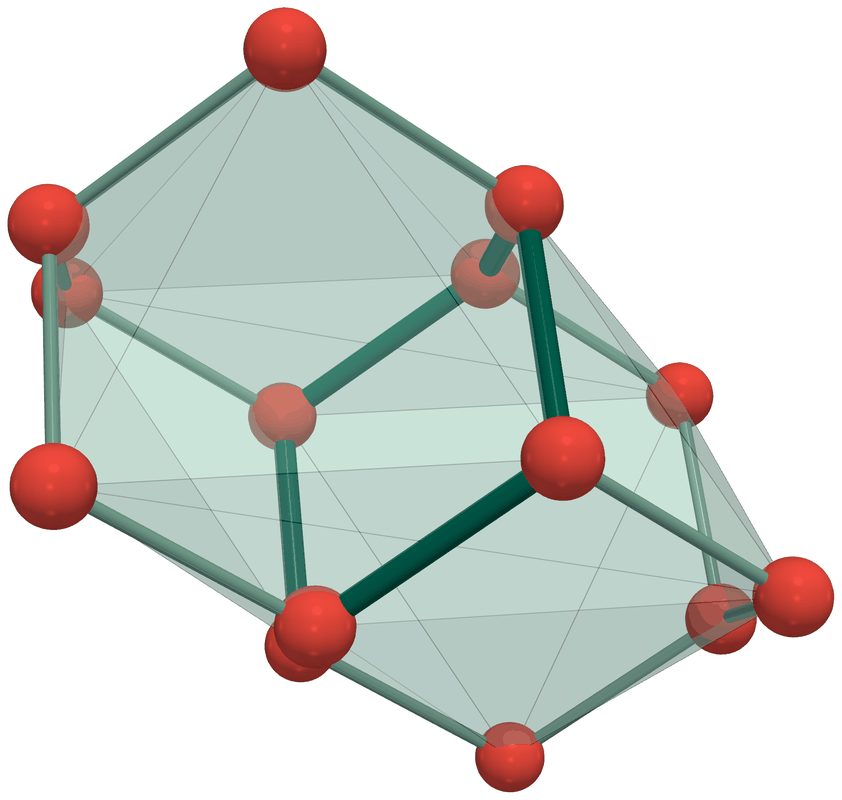
\includegraphics[width=\textwidth]{figures/ddc_cage_solvis_trim}\\[0.4em]
{\small (a)}
\end{minipage}\hfill
\begin{minipage}[t]{0.38\textwidth}
\centering
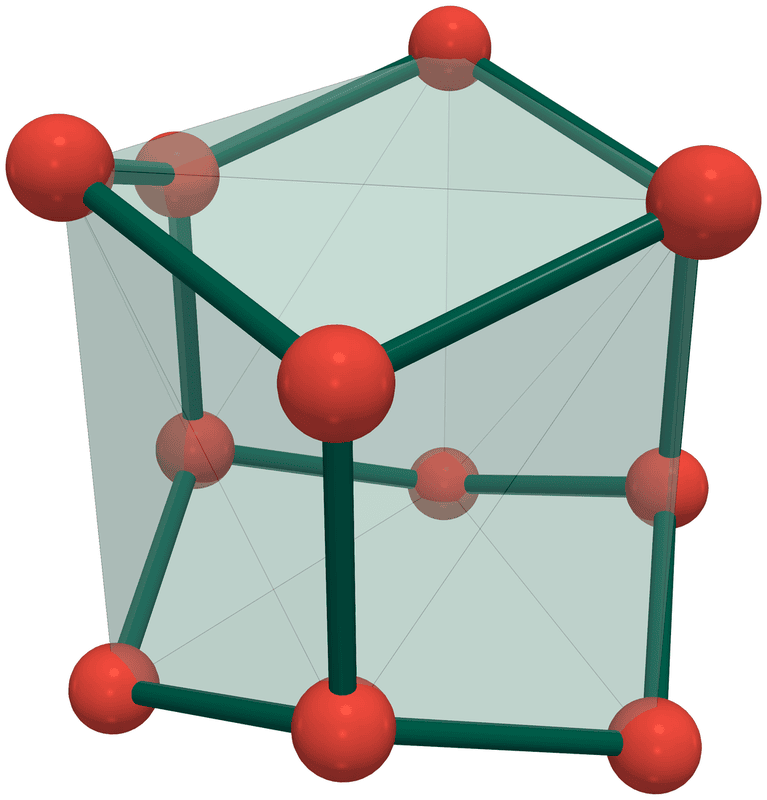
\includegraphics[width=\textwidth]{figures/hc_cage_solvis_trim}\\[0.4em]
{\small (b)}
\end{minipage}
\caption{Topological units rendered with solvis.
(a)~A double-diamond cage (ice Ic) from the first frame of the mW cubic
trajectory. It has fourteen vertices and seven six-rings, and the
equatorial ring is in darker teal. Coordinates are unwrapped about the
cage centroid.
(b)~The twelve-atom hexagonal cage of ice Ih, with two basal hexagons
and the connecting prism faces.}
\label{fig:cages}
\end{figure}

\begin{figure}[htbp]
\centering
\begin{minipage}[t]{0.48\textwidth}
\centering
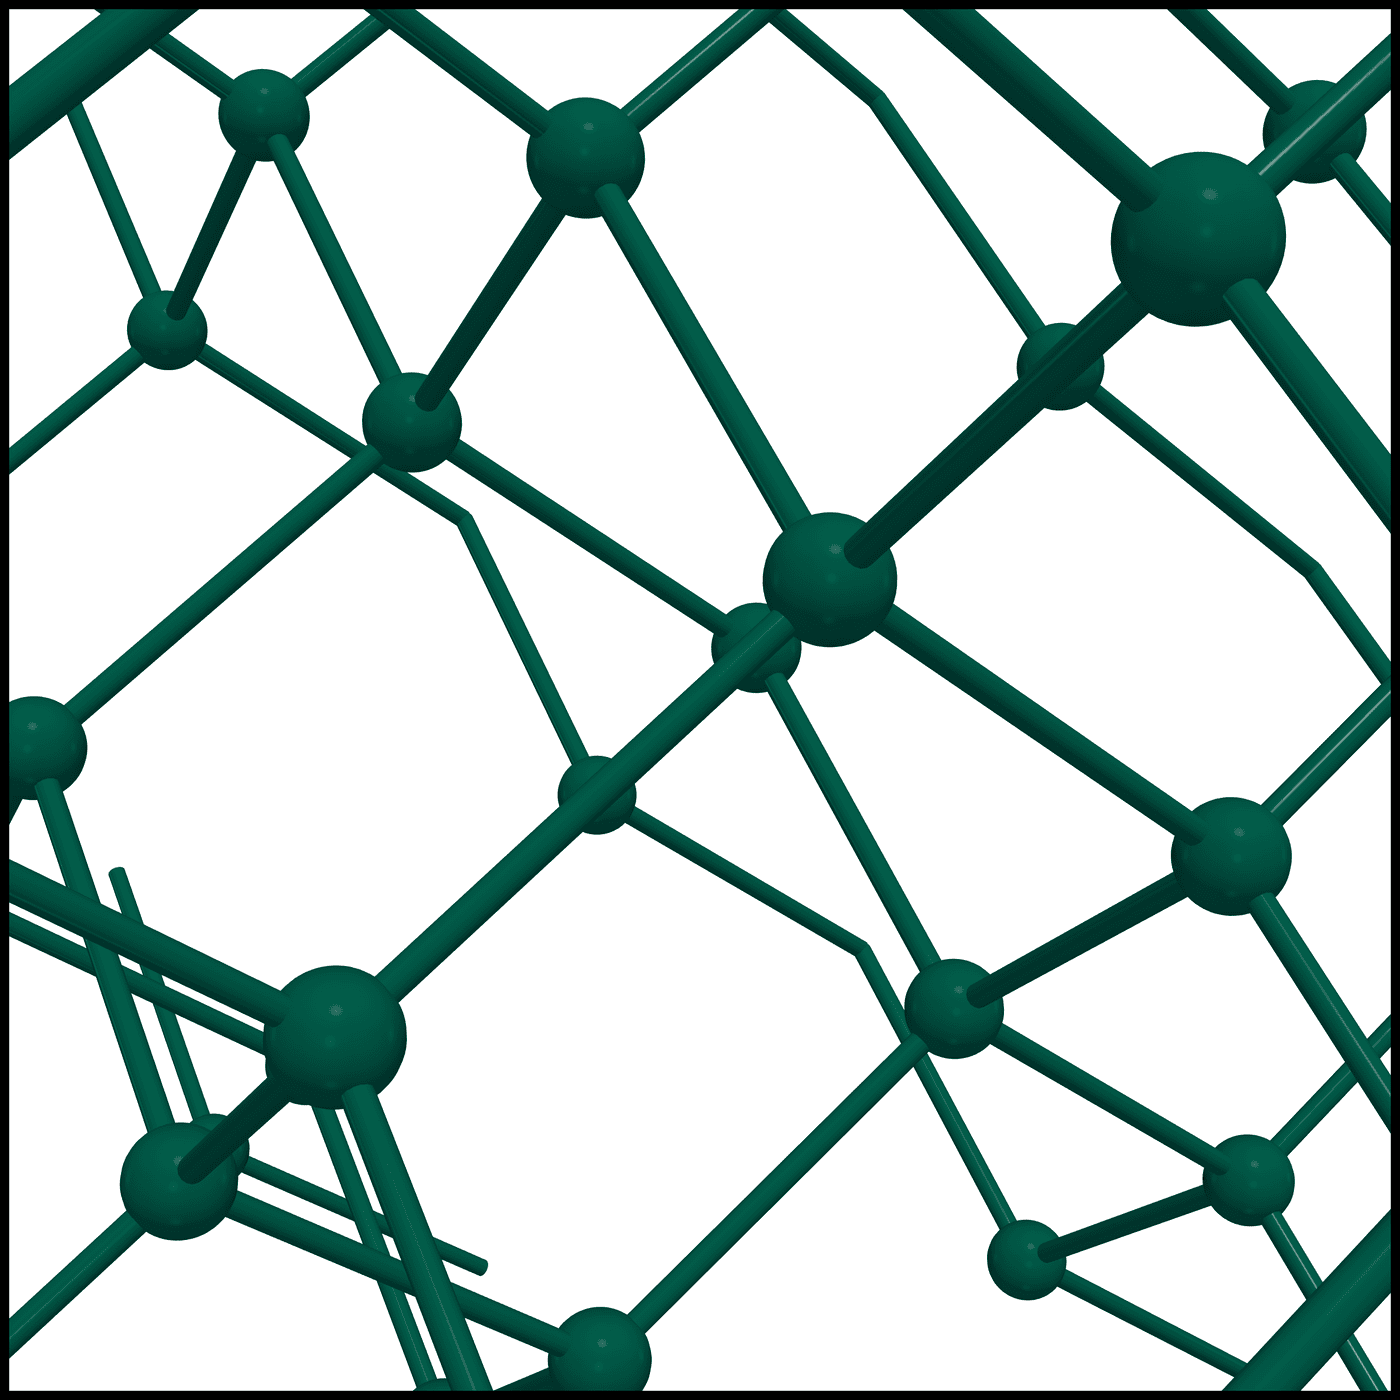
\includegraphics[width=\textwidth]{figures/ic_lattice_solvis_trim}\\[0.3em]
{\small (a)}
\end{minipage}\hfill
\begin{minipage}[t]{0.48\textwidth}
\centering
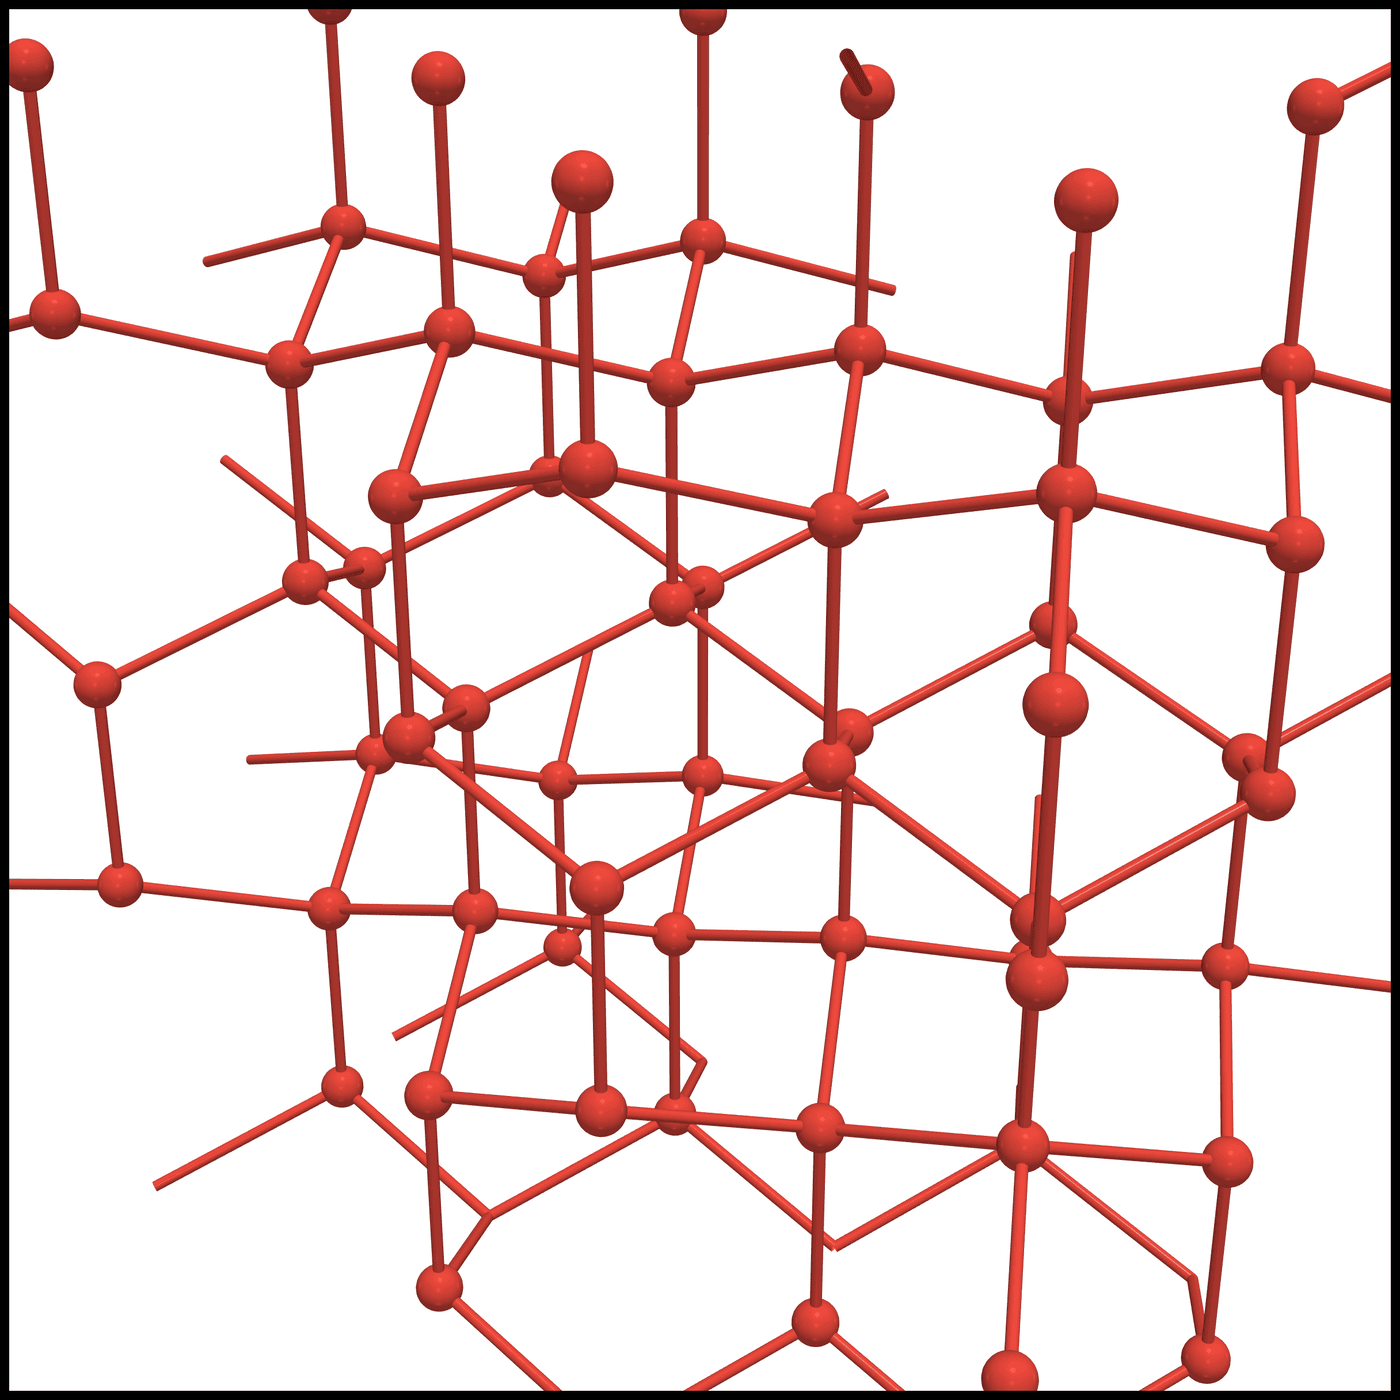
\includegraphics[width=\textwidth]{figures/ih_lattice_solvis_trim}\\[0.3em]
{\small (b)}
\end{minipage}
\caption{Oxygen lattices of ice I, $2\times 2\times 2$ cells, drawn
with solvis.
(a)~Ice Ic (cubic diamond).
(b)~Ice Ih (lonsdaleite), stacked hexagonal layers. Sixty-four
oxygens and first-shell edges in each cell.}
\label{fig:ice-lattices}
\end{figure}

\section{Algorithms}
\label{sec:algorithms}
We build the ring network of a graph and the cage flags on it, and then update both between frames.
Table~\sref{tab:complexity} of the supplement gives the cost of each stage in both versions, and Table~\ref{tab:params} lists the parameters.
Below, \(\Delta\) is the largest degree of \(G\), \(D\) the largest ring size, \(b_r\) the largest \(r\)-hop ball and \(R_6\) the number of six-rings.

\begin{table}[htbp]
\caption{\label{tab:params}Parameters of each analysis and their defaults in seams-core \coretag.
The last column names the command-line option or library call that sets a value; ``fixed'' means none does.}
\centering
\footnotesize
\setlength{\tabcolsep}{3pt}
\begin{tabular}{L{2.1cm}L{3.8cm}L{3.35cm}L{3.6cm}}
analysis & parameter & default & set by\\
\hline
neighbour graphs & cutoff \(r_c\) & \(3.5\,\mathring{\mathrm{A}}\) & \texttt{-{}-cutoff}\\
 & four-nearest \(k\); candidate radius & \(4\); \(r_c+1.5\,\mathring{\mathrm{A}}\) & \texttt{-k}; fixed\\
 & graph of the cage tests & seeded (mutual and union four-nearest) & \texttt{-{}-graph} cutoff, knn, \mbox{knn-union}, seeded\\
primitive rings & largest ring size \(D\) & \(6\) for the cage tests, \(7\) for the fingerprint census & fixed per command\\
 & \(\ell\), \(\ell'\) & \(\lfloor D/2\rfloor\), \(\max(\ell-1,1)\) & from \(D\)\\
ring update & radius \(r\) of \(T\) & \(\max(\lfloor(\ell-2)/2\rfloor,0)\), \(0\) at \(D\le7\) & from \(D\)\\
 & full-pass fraction on \(|X|\) and \(|T|\) & \(0.2\) of \(n\) & C++ only, \texttt{RingUpdater::}\allowbreak\texttt{setFullPassFraction}\\
cage update & batch fraction \(\phi\) on \(|S|/n\) and \(|C|/R_6\) & \(0.25\) & C++ only, \texttt{AffiliationUpdater::}\allowbreak\texttt{setBatchFraction}\\
both updaters & back-off after a whole-frame pass & \(1\), \(2\), \(4\), then at most \(8\) frames & fixed\\
frame range & carry between frames & on for one worker & \texttt{-{}-rebuild}, \texttt{SEAMS\_CARRY=0}\\
CHILL+ & graph & cutoff, \(r_c\) & \texttt{graph} cutoff or mutual in every front end\\
 & staggered and eclipsed \(c_{ij}\) & \(c_{ij}\le-0.8\); \(-0.35\le c_{ij}\le0.25\) & fixed\\
Steinhardt & graph & mutual four-nearest & fixed\\
\end{tabular}
\end{table}

\subsection{Shortest-path ring construction}
\label{sec:org153eae8}
We fix a largest ring size \(D\) and write \(\ell=\lfloor D/2\rfloor\) and \(\ell'=\max(\ell-1,1)\).
For each source \(s\), a breadth-first sweep of \(G\) records the level \(L(v)=d_G(s,v)\) out to \(\ell\) hops.
Vertices of index below \(s\) are dropped, so only the lowest-indexed member of a ring enumerates it.
At each kept vertex \(v\) the sweep stores \(\Pi(v)\), the shortest \(s\)--\(v\) paths whose vertices are all at least \(s\).
At each vertex \(p\) with \(1\le L(p)\le\ell\), pairs of stored paths close the candidates of Eq.~\ref{eq:yuan}.
Two paths in \(\Pi(p)\) with disjoint interiors close an even ring of size \(2L(p)\).
A neighbour \(q>p\) of \(p\) on the same level closes an odd ring of size \(2L(p)+1\) with one path to each.
A candidate is kept when it satisfies Eq.~\ref{eq:franzblau}.
The test reads rows \(d_{\ell'}(u,\cdot)\) of radius \(\ell'\), computed once per frame, and a missing entry counts as greater than \(\ell'\).
A shortcut between two members of a candidate of size at most \(D\) has at most \(\ell'\) edges, so the rows decide Eq.~\ref{eq:franzblau} exactly.
We prove in Proposition~\sref{prop:alg1} of the supplement that Algorithm~\ref{alg:rings} emits every primitive ring of size at most \(D\) once and nothing else.
The test suite checks that its ring set equals that of the walk enumeration of d-SEAMS 1, which the library keeps.

\begin{algorithm}[htbp]
\caption{Primitive rings from shortest-path pairs}
\label{alg:rings}
\begin{algorithmic}[1]
\Require graph \(G=(V,E)\), \(V=\{0,\ldots,n-1\}\); largest ring size \(D\)
\Ensure every primitive ring with \(3\le|R|\le D\), once, from its lowest-indexed member (Proposition~\sref{prop:alg1})
\State \(\ell\gets\lfloor D/2\rfloor\); \(\ell'\gets\max(\ell-1,1)\)
\State \(d_{\ell'}(u,\cdot)\gets\) breadth-first distances to \(\ell'\) hops, for every \(u\in V\)
\ForAll{\(s\in V\)} \Comment{independent sources}
  \State \(L(\cdot)\gets\) breadth-first levels from \(s\) on \(G\) to depth \(\ell\); drop every \(v<s\)
  \State \(\Pi(v)\gets\) shortest \(s\)--\(v\) paths of \(G\) through vertices \(\ge s\), for each kept \(v\)
  \ForAll{\(p\) with \(1\le L(p)\le\ell\)}
    \If{\(3\le 2L(p)\le D\)}
      \ForAll{\(P<P'\) in \(\Pi(p)\) with disjoint interiors}
        \State \Call{Keep}{$(s,P,p,P'^{-1})$} \Comment{even ring, Eq.~\ref{eq:yuan}}
      \EndFor
    \EndIf
    \If{\(2L(p)+1\le D\)}
      \ForAll{\(q\in N(p)\), \(q>p\), \(L(q)=L(p)\); \(P\in\Pi(p)\), \(Q\in\Pi(q)\), interiors disjoint and off \(p,q\)}
        \State \Call{Keep}{$(s,P,p,q,Q^{-1})$} \Comment{odd ring closed by \(pq\)}
      \EndFor
    \EndIf
  \EndFor
\EndFor
\Function{Keep}{$C$}
  \State emit \(C\) if \(d_{\ell'}(c_i,c_j)\ge d_C(c_i,c_j)\) for all \(i<j\) \Comment{Eq.~\ref{eq:franzblau}; absent means \(>\ell'\)}
\EndFunction
\end{algorithmic}
\end{algorithm}

With \(P_s\) stored paths and \(K_s\) inspected path tuples at source \(s\), the pass costs \(O\bigl(n\,\Delta\,b_{\ell'}+\sum_s(\Delta b_\ell+\ell P_s+D^2K_s)\bigr)\), linear in \(n\) at fixed \(\Delta\) and \(D\) (Section~\sref{sec:s-costs}).

\subsection{Locality and the ring update}
\label{sec:orgab1f013}
We write \(G\cup G'\) for the union of the graphs of two consecutive frames, \(\Delta E\) for the symmetric difference of their edge sets and \(X\) for the endpoints of \(\Delta E\), the atoms whose neighbour row changed.
A cycle of at most \(D\) members that holds no edge of \(\Delta E\) is a cycle of both graphs.
It is a primitive ring of one and not of the other only if a changed edge lies on a shortcut, a path of fewer than \(\ell\) edges between two of its members.
One endpoint of that edge then lies within \(r=\max(\lfloor(\ell-2)/2\rfloor,0)\) edges of a member.
Every ring of size at most \(D\) that differs between the frames therefore meets
\begin{equation}
T=\bigl\{v:d_{G\cup G'}(v,X)\le r\bigr\},
\label{eq:hopbound}
\end{equation}
and for \(D\le 7\) \(T\) is \(X\) itself (Proposition~\sref{prop:alg2}, Figure~\sref{fig:hopbound}).
A coarser test, which the engine does not use, follows from the ball a source reads.
Every member of a ring that \(s\) enumerates lies within \(\ell\) hops of \(s\), so a source more than \(2\ell-1\) hops from \(X\) keeps its rings (Proposition~\sref{prop:local} and Corollary~\sref{cor:source}).
The bound is a statement about \(G\cup G'\), not a numerical tolerance.

The updater stores the sorted ring list of the previous frame (Algorithm~\ref{alg:hopbound}).
On a new frame it refreshes the distance rows within \(\ell'\) of \(X\) and drops the stored rings that meet \(T\).
From each \(s\in T\) it enumerates on \(G'\) the rings through \(s\) whose lowest-indexed member in \(T\) is \(s\), and merges them into the kept rings.
The merged list equals a full rebuild (Proposition~\sref{prop:alg2}).
At fixed churn the fraction of atoms in \(T\) falls as \(1/n\).

\begin{algorithm}[htbp]
\caption{Hop-bound ring update between frames}
\label{alg:hopbound}
\begin{algorithmic}[1]
\Require stored rings \(\mathcal{R}\) of \(G\), sorted, and rows \(d_{\ell'}\) of \(G\); the next graph \(G'\)
\Ensure \(\mathcal{R}\) for \(G'\), equal to Algorithm~\ref{alg:rings} on \(G'\) (Proposition~\sref{prop:alg2})
\State \(X\gets\{v:N'(v)\ne N(v)\}\) \Comment{endpoints of \(\Delta E\), by sorted neighbour rows}
\If{\(X=\emptyset\)}
  \State \Return \(\mathcal{R}\)
\EndIf
\State \(T\gets\{v: d_{G\cup G'}(v,X)\le r\}\), \(r=\max(\lfloor(\ell-2)/2\rfloor,0)\) \Comment{Eq.~\ref{eq:hopbound}; \(T=X\) for \(D\le7\)}
\If{\(|X|>\lfloor0.2n\rfloor\) or \(|T|>\lfloor0.2n\rfloor\)}
  \State \Return Algorithm~\ref{alg:rings} on \(G'\) \Comment{one pass over every source}
\EndIf
\State \(U\gets\{u: d_{G\cup G'}(u,X)\le\ell'\}\); recompute \(d_{\ell'}(u,\cdot)\) on \(G'\) for \(u\in U\) \Comment{Proposition~\sref{prop:rows}}
\State \(\mathcal{A}\gets\emptyset\)
\ForAll{\(s\in T\)}
  \State \(\mathcal{A}\gets\mathcal{A}\,\cup\) Algorithm~\ref{alg:rings} from \(s\) on \(G'\), dropping only the vertices of \(T\) below \(s\)
\EndFor
\State \Return \(\{R\in\mathcal{R}:R\cap T=\emptyset\}\cup\mathcal{A}\), sorted \Comment{merge of two sorted lists}
\end{algorithmic}
\end{algorithm}

The local work is linear in \(|\Delta E|\) at fixed \(\Delta\) and \(D\), and the merge reads every stored ring on every frame (Section~\sref{sec:s-costs}).
The Lean statements S14--S16 check the ball agreement and the case split of the source bound for an abstract local enumerator; they model neither Algorithm~\ref{alg:rings} nor the set \(T\).

\subsection{Inverted index and cage search}
\label{sec:orgf57a77e}
Both cage tests ask which six-rings contain a given atom.
Scanning the ring list for each question is quadratic in the ring count.
One pass builds
\begin{equation}
I(v)=\bigl\{R:v\in R\bigr\},
\label{eq:index}
\end{equation}
with each row in ascending ring order, and answers the question in time linear in the number of rings through \(v\).
Both \(\beta(R,R')\) and \(\beta(R',R)\) bond \(l_0\) or \(l_1\) to an atom of \(R'\), so the HC search draws the partners of \(R\) from the rows of the neighbours of \(l_0\) and \(l_1\).
The equator tests of Eqs.~\ref{eq:ddc1} and \ref{eq:ddc2} are intersections of the rows of the candidate's vertices.
The prismatic rings of an HC are the same intersection against the two basals (Algorithm~\ref{alg:cages}).

\begin{algorithm}[htbp]
\caption{Hexagonal and double-diamond cages from the inverted index}
\label{alg:cages}
\begin{algorithmic}[1]
\Require primitive six-rings \(\mathcal{R}_6\); neighbour rows \(N(\cdot)\)
\Ensure the flags \(\alpha_{\mathrm{HC}}(R)\) and \(\alpha_{\mathrm{DDC}}(R)\) of Eqs.~\ref{eq:ddc-aff} and \ref{eq:ice}
\State \(I(v)\gets\{R\in\mathcal{R}_6:v\in R\}\), each row ascending \Comment{Eq.~\ref{eq:index}}
\ForAll{\(R=(r_0,\ldots,r_5)\in\mathcal{R}_6\)} \Comment{basal pairs}
  \ForAll{\(R'\ne R\) in \(\bigcup_{u\in N(r_0)\cup N(r_1)}I(u)\)}
    \If{\(\beta(R,R')\)}
      \State \(\alpha_{\mathrm{HC}}\gets\) true on \(R\), \(R'\) and the rings of \(\bigcup_{v\in R\cup R'}I(v)\) prismatic to the pair
    \EndIf
  \EndFor
\EndFor
\ForAll{\(R\in\mathcal{R}_6\) with \(\neg\alpha_{\mathrm{HC}}(R)\)} \Comment{HC rings are not equators}
  \If{\(|I(r_k)|\ge 4\) for \(k=0,\ldots,5\)} \Comment{Eq.~\ref{eq:ddc1}}
    \State \(T_k\gets I(r_k)\cap I(r_{k+1})\cap I(r_{k+2})\setminus\{R\}\), indices mod 6 \Comment{Eq.~\ref{eq:ddc2}}
    \If{every \(T_k\ne\emptyset\)}
      \If{some six distinct \(R'_k\in T_k\) pass the alternating-intersection conditions for some \(j\)}
        \State \(\alpha_{\mathrm{DDC}}\gets\) true on \(R\) and on every ring of \(P(R)\)
      \EndIf
    \EndIf
  \EndIf
\EndFor
\end{algorithmic}
\end{algorithm}

Both passes are linear in \(R_6\) at fixed degree, where the pair scans of d-SEAMS 1 were \(O(R_6^2)\), and on ice Ic \(R_6=2n\) (Section~\sref{sec:s-costs}).
Cage objects, as opposed to flags, need an order in which rings are claimed.
Both searches visit rings in the order of their position-keyed atom ranks, so the cage objects do not depend on the atom labels or the order of the ring list (Section~\sref{sec:s-invariance}).

\subsection{Incremental cage affiliation}
\label{sec:affupdate}
The flags admit an incremental update because they claim nothing.
We call two six-rings adjacent when one contains an atom within one bond of an atom of the other, and write \(A(R)\) for the six-rings adjacent to \(R\).
A basal partner of \(R\) bonds an atom to \(R\), so it lies in \(A(R)\), and \(\beta\) reads only the two rings and the rows of their atoms.
A prismatic ring shares atoms with both basals, so both lie in its adjacency set.
The equator tests for \(R\) read the rings that share an atom with \(R\) and \(\alpha_{\mathrm{HC}}(R)\).
A peripheral shares an atom with its equator.
Hence \(\alpha_{\mathrm{HC}}(R)\) is a function of the rings in \(A(R)\) and the rows of their atoms, and \(\alpha_{\mathrm{DDC}}(R)\) of the rings in \(A(A(R))\) and their rows.

Between two frames a flag can change only on a ring whose second adjacency set touches an added ring, a removed ring, or an atom whose neighbour row changed.
We write \(S\) for the atoms of those three kinds.
Write \(X(S)\) for the rings through an atom of \(S\) or a neighbour of one, \(I(S)\) for the rings through an atom of \(S\), and \(Y(Q)\) for the rings that share an atom with a ring of \(Q\).
The rings whose flags can change are then
\begin{equation}
C=Y\bigl(X(S)\cup Y(I(S))\bigr),
\label{eq:dirty}
\end{equation}
and every ring outside \(C\) keeps the flags of its match in the previous frame.
Algorithm~\ref{alg:affupdate} computes \(C\), carries every other flag and evaluates the tests of Algorithm~\ref{alg:cages} only where they can set a flag on \(C\).
We match rings across frames by a hash of each canonical cycle and confirm each match atom by atom.

\begin{algorithm}[htbp]
\caption{Incremental cage affiliation between frames}
\label{alg:affupdate}
\begin{algorithmic}[1]
\Require flags \(\alpha_{\mathrm{HC}},\alpha_{\mathrm{DDC}}\), sorted rows \(N\) and six-rings \(\mathcal{R}_6\) of the previous frame; rows \(N'\) and six-rings \(\mathcal{R}'_6\) of the next; \(\phi=0.25\)
\Ensure the flags of Algorithm~\ref{alg:cages} on \((\mathcal{R}'_6,N')\)
\State \(S\gets\{v:N'(v)\ne N(v)\}\) \Comment{changed rows}
\If{\(|S|\,R_6>\lfloor\phi R_6\rfloor\,n\)}
  \State \Return Algorithm~\ref{alg:cages} on \((\mathcal{R}'_6,N')\)
\EndIf
\If{\(S=\emptyset\) and \(\mathcal{R}'_6=\mathcal{R}_6\) in order}
  \State \Return the stored flags
\EndIf
\State \(I\gets\) inverted index of \(\mathcal{R}'_6\) \Comment{Eq.~\ref{eq:index}}
\State match \(\mathcal{R}'_6\) to \(\mathcal{R}_6\) by cycle hash, confirmed atom by atom
\State \(S\gets S\,\cup\) atoms of the added and the removed rings
\State \(C\gets Y\bigl(X(S)\cup Y(I(S))\bigr)\) \Comment{Eq.~\ref{eq:dirty}}
\If{\(|C|>\lfloor\phi R_6\rfloor\)}
  \State \Return Algorithm~\ref{alg:cages} on \((\mathcal{R}'_6,N')\)
\EndIf
\State copy \(\alpha_{\mathrm{HC}},\alpha_{\mathrm{DDC}}\) of each ring outside \(C\) from its match
\State HC tests of Algorithm~\ref{alg:cages} on the rings within one bond of \(C\); set flags on \(C\) only
\State DDC tests on the rings that share an atom with \(C\); set flags on \(C\) only
\State \Return the flags
\end{algorithmic}
\end{algorithm}

An incremental update costs the sorted row diff, the ring diff, the index and the tests near \(C\) (Section~\sref{sec:s-costs-cage}).
The Catch2 case ``AffiliationUpdater tracks synthetic topology churn exactly'' and the trajectory benchmarks of Section~\ref{sec:incremental} compare it with Algorithm~\ref{alg:cages} on every frame.

Both updaters fall back to a whole-frame pass when most of a frame changes, and on such a frame the diff they computed first is spent for nothing.
After a frame that falls back, each updater runs the whole-frame pass with no diff for the next 1, 2, 4 and then at most 8 frames.
A frame on which the diff wins resets the wait.
Every pass is exact, so this back-off changes only the cost.
The two fractions are \(0.2\) and \(\phi=0.25\) (Table~\ref{tab:params}).
In the C++ library of \coretag{}, \texttt{RingUpdater::setFullPassFraction} and \texttt{AffiliationUpdater::setBatchFraction} set them.
The command line and PydSEAMSlib~2.11.1 run both updaters at these defaults.

\subsection{Carrying rings and cages through a trajectory}
\label{sec:carry}
The \texttt{seams} command line holds one ring updater for each graph and ring size and one affiliation updater for each graph, and it passes every frame of a range through them (Figure~\sref{fig:carry}).
The seeded label reads the mutual and the union four-nearest graphs, so it holds two of each.
A one-worker range on a LAMMPS dump carries them between consecutive frames, and so does any range on the serial chemfiles and readcon readers.
Frame-parallel workers, MPI ranks and single frames rebuild every frame, because their frames do not reach one thread in order.
\texttt{-{}-rebuild} or \texttt{SEAMS\_CARRY=0} switches the carry off.
The Meson test \texttt{seams\_carried\_frames\_match\_rebuild} compares the JSON output of a carried range with the three rebuilt paths on three trajectories, and every output is identical (Section~\sref{sec:s-carry}).

\section{Benchmarks}
\label{sec:benchmarks}
\subsection{Machines and protocol}
\label{sec:protocol}
Every timing names its record, a directory under \texttt{repro-records/} of the supplementary data (Table~\sref{tab:records} of the supplement).
Every record runs seams-core \coretag{}, source tree \coretree, built from the program-files archive, and each \texttt{run.sh} refuses a tree that differs from that archive.
The machine is a KVM guest with 8 vCPUs on an Intel Xeon of CPUID family 6 and model 207.
We time on its pinned core 3 with \texttt{OMP\_NUM\_THREADS=1}.
The d-SEAMS 1 baseline is seams-core commit \texttt{1c8efa38} (2026-05-28).
It keeps the walk enumeration, the pair-scan HC search followed by the DDC search, and the all-pairs index-ordered neighbour builder of the 2020 release.
A driver timing is a \texttt{std::chrono::steady\_clock} interval around the library call with the frame already in memory.
Section~\sref{sec:s-protocol} of the supplement gives the machine, the builds and the repetition rules.

\subsection{One frame against d-SEAMS 1}
\label{sec:oneframe}
We time both versions on pinned core 3 (record \texttt{bench-2026-10-31}) on the 4096-molecule mW cubic frame, which has 8192 six-rings, as the best of five calls per stage.
Each stage has its own timer in both versions.
\texttt{findHC} is timed alone, and \texttt{findDDC} is timed alone on the ring types and cages that \texttt{findHC} leaves, restored outside the timer before each call.
The path is the sum of the three timers in one session, and we give the session whose path is the median of the three.
There the baseline takes \(75.072\,\mathrm{ms}\) in ring detection, \(2565.070\,\mathrm{ms}\) in \texttt{findHC} and \(224.142\,\mathrm{ms}\) in \texttt{findDDC}, \(2864.284\,\mathrm{ms}\) in all.
In 2.0 the three take \(3.504\), \(40.798\) and \(2.519\,\mathrm{ms}\), \(46.821\,\mathrm{ms}\) in all, a factor of \(61.2\) (Figure~\ref{fig:pipeline}).
Both versions assign none of the 8192 six-rings to an HC and every one to a DDC, and they return 1955 and 2040 DDC objects in two visiting orders (Section~\sref{sec:s-bench}).
Section~\sref{sec:s-bench} of the supplement also gives the ring scaling, the neighbour lists, the OpenMP strong scaling and the same rows on two Elja nodes.

\begin{figure}[htbp]
\centering
\resizebox{\textwidth}{!}{\input{figures/pipeline}}
\caption{Ring-and-cage wall time on the 4096-molecule mW cubic frame
(8192 six-rings), pinned core 3 of the cloud VM, record \texttt{bench-2026-10-31},
best of five calls per stage in the session whose path is the median of three.
Baseline (commit \texttt{1c8efa38}) is walk enumeration and pair scans.
2.0 (seams-core \coretag) is shortest-path rings and the inverted-index searches.
In both versions each bar is the timer of one stage, with \texttt{findHC} and \texttt{findDDC} timed alone, and the path is the sum of the three
($2864\,\mathrm{ms}$ and $46.8\,\mathrm{ms}$).}
\label{fig:pipeline}
\end{figure}

\subsection{Incremental updates}
\label{sec:incremental}
On a jittered 8000-molecule cell with three perturbed sites per frame the ring update matches a full rebuild on each of five frames.
The smallest update over the five takes \(1.477\,\mathrm{ms}\) against a smallest rebuild of \(28.839\,\mathrm{ms}\) (record \texttt{bench-2026-10-31}).
On the eleven stored frames of the 4096-molecule mW cubic trajectory no bond of the mutual four-nearest graph changes after the first, so \(X\) is empty and no ring can change.
The ring update then returns the stored network in \(0.170\,\mathrm{ms}\) against \(3.316\,\mathrm{ms}\) for a rebuild, and the affiliation update returns its flags in \(0.273\,\mathrm{ms}\) against \(38.376\,\mathrm{ms}\) (Figure~\sref{fig:incremental}).
Both equal the rebuild on every frame.

We measure the cost against the size of a change with \texttt{tests/}\allowbreak\texttt{bench\_churn\_sweep.cpp}, a driver new in \coretag{} (file \texttt{churn-sweep-}\allowbreak\texttt{1t.txt} of the record, median of seven repetitions, one thread).
It starts from frame 147 of the figshare mW nucleation excerpt (4096 molecules, cutoff graph) and moves the molecules within a radius of the box centre to their frame-148 positions.
With 3 changed bonds the ring update takes \(0.340\,\mathrm{ms}\) against \(12.878\,\mathrm{ms}\) for a rebuild, and the affiliation update \(1.880\,\mathrm{ms}\) against \(18.537\,\mathrm{ms}\) for the batch pass.
With 208 changed bonds the two take \(1.892\) against \(13.018\,\mathrm{ms}\) and \(4.377\) against \(18.176\,\mathrm{ms}\).
The ring update is faster than the rebuild at every point up to 867 changed bonds, where it takes \(6.054\) against \(12.914\,\mathrm{ms}\).
At 1348 changed bonds 1018 atoms change, more than \(\lfloor 0.2\cdot 4096\rfloor=819\), and the updater switches to the full pass.
From 340 changed bonds the affiliation update exceeds its batch fraction \(\phi=0.25\) and switches to the batch pass.
Past either switch the rebuild is the faster call, since the updater pays for its diff before the same pass, and the update takes at most \(3.1\%\) longer than the rebuild at any point of the sweep.
Every point of the sweep equals the batch computation.
The reproducibility package runs the same driver as an asv suite under Snakemake (Section~\sref{sec:s-repro}).

The saved frames of deposited nucleation runs change far more.
On frames 2--11 of the excerpt 2845 bonds change per frame on average, and 1948 on frames 2--11 of Niu trajectory 3 (2880 molecules) \citep{niu2019temperature}.
Both updaters then take the batch pass on every frame.
On one core the ring update takes \(13.491\) against \(12.997\,\mathrm{ms}\) and the affiliation update \(14.925\) against \(14.791\,\mathrm{ms}\) on the excerpt, and \(9.784\) against \(9.681\,\mathrm{ms}\) and \(8.635\) against \(8.557\,\mathrm{ms}\) on Niu trajectory 3 (one session).
Over all 147 frames of the excerpt after the first, 67.15\% of the molecules change their row per frame (record \texttt{incremental-md-}\allowbreak\texttt{2026-10-31}).
There the ring update takes \(1997.386\) against \(1946.342\,\mathrm{ms}\) for the rebuilds, 2.6\% longer, and the affiliation update \(2454.199\) against \(2457.197\,\mathrm{ms}\).
We also ran 168 mW trajectories for the purpose, with eleven frames saved every 1 to 100 steps.
On ice neither updater switches, and the ring update takes \(1.899\) to \(5.726\,\mathrm{ms}\) against \(37.538\) to \(47.553\,\mathrm{ms}\) for a rebuild (record \texttt{incremental-md-2026-10-31}, Section~\sref{sec:s-incremental}).

We time the whole command line, \texttt{seams cages} over a frame range on pinned core 3, with the carry and with \texttt{-{}-rebuild} (record \texttt{cli-carry-}\allowbreak\texttt{2026-10-31}, Table~\sref{tab:carry}).
Each case runs in five alternating sessions, and the carried and rebuilt JSON outputs are identical byte for byte in every case.
On the mW crystal the carried walk is 6.38 times faster per frame on the seeded graph and 5.41 times on the cutoff graph.
On the two deposited trajectories the ratio lies between 0.981 and 1.038, so the carried walk is at most 1.9\% slower than the rebuild.

\subsection{Comparison with existing codes}
\label{sec:comparison}
We time the computations that d-SEAMS 2.0 shares with another code on the same frames and core, and compare the outputs (Table~\ref{tab:compare}).
Every code reads the same oxygen coordinates and orthorhombic cell, and every library runs on one thread.
Each timer holds the neighbour search of its code, except in the \(q_6\) rows.
There both codes read one mutual four-nearest list, which d-SEAMS builds once outside both timers.
The frames are the 4096-molecule mW cubic frame, the final frame of the 2880-water Niu dump and the 1000-molecule continuous random network CRN1.
The others are the \(2\times2\times2\) GenIce sI framework of 368 waters and a 512-molecule ice Ic lattice with Gaussian jitter \(\sigma=0.3\,\mathring{\mathrm{A}}\) (generator seed 5).
Section~\sref{sec:s-h2h} of the supplement lists the calls on each side.

\begin{table}[htbp]
\caption{\label{tab:compare}Single-core timings in milliseconds on the same frames, record \texttt{h2h-2026-10-31}.
The machine is an 8-vCPU KVM guest on an Intel Xeon of CPUID family 6 and model 207, timed on pinned core 3 with \texttt{OMP\_NUM\_THREADS=1}, best of seven runs after one warm-up.
The codes are OVITO 3.15.5 \citep{stukowski2010visualization,ovito315}, freud 3.5.0 \citep{ramasubramani2020freud}, GenIce2 2.2.13.3 \citep{matsumoto2018genice} with cycless 0.7 and genice2-cage 2.5.2, and RINGS 1.3.5 \citep{leroux2010rings}.
The d-SEAMS side is seams-core \coretag{} through its command line and PydSEAMSlib 2.11.1 built on it.
Agreement compares the two outputs; the \(q_6\) rows give the largest difference of \(q_6\) and \(\bar q_6\).
In the CNA rows a diamond atom and its first and second neighbours count as that phase.
The mW RINGS rows are n=3: three recorded repetitions and no further warmup, run at the same time with one repetition pinned to each of cores 3, 4 and 5. The d-SEAMS repetitions used those same cores and finished before RINGS started. The CRN1 rows are unchanged.
The PTM row is the median of 30 repetitions after five warm-ups, from \texttt{scripts/ptm\_rows.py}, not the best of seven.
Its d-SEAMS time is \texttt{bench\_paper} in mode \texttt{seeded-adj}.}
\centering
\scriptsize
\setlength{\tabcolsep}{2.6pt}
\begin{tabular}{L{2.75cm}L{2.15cm}L{1.85cm}>{\raggedleft\arraybackslash}p{1.4cm}>{\raggedleft\arraybackslash}p{1.62cm}L{2.35cm}}
computation & frame & other code & d-SEAMS 2.0 & other & agreement\\
\hline
CHILL+ labels, cutoff list & mW cubic, 4096 & OVITO & 6.20 & 22.6 & 4096 of 4096\\
CHILL+ labels, cutoff list & Niu final frame, 2880 & OVITO & 5.30 & 21.2 & 2610 of 2880\\
\(q_6\), \(\bar q_6\), one mutual four-nearest list & mW cubic, 4096 & freud & 1.27 & 35.1 & \(1.6\times10^{-7}\)\\
\(q_6\), \(\bar q_6\), one mutual four-nearest list & Niu final frame, 2880 & freud & 0.897 & 24.7 & \(1.1\times10^{-5}\)\\
Ic/Ih labels; seeded cages, CNA & mW cubic, 4096 & OVITO identify diamond & 110 & 5.69 & 4096 of 4096\\
Ic/Ih labels; seeded cages, CNA & Niu final frame, 2880 & OVITO identify diamond & 70.8 & 4.95 & 1763 of 2880\\
Ic/Ih labels; seeded cages, CNA & jittered Ic, 512 & OVITO identify diamond & 15.0 & 0.798 & 508 of 512\\
Ic/Ih labels; completed cages, PTM & jittered Ic, 512 & OVITO PTM & 7.106 & 16.306 & 512 and 52 Ic\\
primitive rings, \(D=6\), ring stage (n=3) & mW cubic, 4096 & RINGS & 6.735 & 52190 & same census, 8192 rings\\
primitive rings, \(D=6\), ring stage & CRN1, 1000 & RINGS & 2.76 & 3770 & same census, 1238 rings\\
primitive rings, \(D=6\), whole process (n=3) & mW cubic, 4096 & RINGS & 69.500 & 3694790.404 & same census\\
primitive rings, \(D=6\), whole process & CRN1, 1000 & RINGS & 13.8 & 138608 & same census\\
shortcut-free rings, \(D=6\) & mW cubic, 4096 & GenIce2 & 7.46 & 11390 & same 8192 rings\\
shortcut-free rings, \(D=6\) & CRN1, 1000 & GenIce2 & 2.80 & 1881 & same 1238 rings\\
\(5^{12}\) and \(5^{12}6^{2}\) cages & sI, 368 & GenIce2 & 3.81 & 487 & 16 and 48 in both\\
\end{tabular}
\end{table}

On one core the d-SEAMS CHILL+ call is 3.6 and 4.0 times faster than OVITO's.
On one shared list its \(q_6\) call is 28 times faster than freud's on both frames.
Its ring search is 1500 and 670 times faster than that of cycless, and its cage search 130 times faster than that of GenIce2, with the same ring vertex sets and the same cage counts.
RINGS returns the same census of primitive rings by size as d-SEAMS.
On the mW frame the recorded medians are 6.735~ms against 52190~ms for the ring stage and 69.500~ms against 3694790.404~ms for the whole process.
The printed three-decimal medians give a ring-stage ratio 52190.000/6.735 = 7749.07 and a whole-process ratio 3694790.404/69.500 = 53162.5, about \(5.3\times10^{4}\).
The unrounded medians give 52190/6.73451 = 7749.64 and 3694790.404052/69.499658 = 53162.71.
On CRN1 the ring stage still takes 1400 times as long as the d-SEAMS ring call.
The identify-diamond modifier of OVITO, a common-neighbour analysis, labels Ic and Ih in 19, 14 and 19 times less time than the seeded cage label on the three frames.
The two agree on every mW molecule, at 508 of the 512 jittered sites and at 1763 of the 2880 Niu molecules.
The CHILL+ labels agree on every mW molecule and differ at 270 Niu molecules, 109 of which d-SEAMS labels interfacial clathrate and OVITO other.

\subsection{Label accuracy}
\label{sec:accuracy}
None of the other codes returns an HC or DDC label.
We measure those labels against CHILL+, polyhedral template matching (PTM) and the Steinhardt rules on ice Ic (512 sites) and ice Ih (360 sites) under a Gaussian displacement of \(\sigma\) per component (Figure~\ref{fig:sota}, record \texttt{sota-heldout-2026-10-31}).
At \(\sigma=0.3\,\mathring{\mathrm{A}}\) the cutoff graph keeps \(0.936\) and \(0.899\) of the Ic and Ih sites, the seeded rule \(0.999\) and \(0.994\), PTM \(0.089\) and \(0.099\) and CHILL+ \(0.564\) and \(0.567\).
At \(0.4\,\mathring{\mathrm{A}}\) the seeded rule keeps \(0.698\) and \(0.589\), and ring completion raises those to \(0.942\) and \(0.728\).
On a 360-point random packing no cage rule and no PTM label marks any molecule, and on a 512-molecule mW liquid at \(215\,\mathrm{K}\) the seeded rules label \(0.023\) of the molecules Ic or Ih.
Section~\sref{sec:s-accuracy} of the supplement gives the full table, the held-out mW trajectories and the definitions of the rules.

\begin{figure}[htbp]
\centering
\resizebox{\textwidth}{!}{\input{figures/sota_acc}}
\caption{Lattice-label retention of ice Ic and ice Ih under a
Gaussian displacement $\sigma$ per component (Table~\sref{tab:sota});
points are means over realizations 5 to 9, bars their range. At
$0.4\,\mathring{\mathrm{A}}$ the seeded rule keeps $0.70$ and $0.59$,
the cutoff graph $0.35$ and $0.23$, template matching $0.000$ and
$0.000$ and CHILL+$(r_c)$ $0.10$ and $0.10$. No cage assignment
labels any molecule of the null.}
\label{fig:sota}
\end{figure}

\subsection{Reproduction}
\label{sec:repro}
The reproducibility package is
\url{https://github.com/d-SEAMS/dseams2_repro} \citep{dseams2repro},
at commit \texttt{\reprobase} (tag v2.7.0).
The records dated 31 October 2026 ran on that commit with the first revision of the package patch (sha256 \texttt{0e53bc8e}, tree \texttt{5dde84a5}).
The revision cited here (sha256 \texttt{f5328ee6}, tree \texttt{7863e79e}) adds the PTM cutoff 0.1 and \texttt{scripts/ptm\_cutoff\_sweep.py}.
The 0.1 PTM rows ran on it.
The patch adds the program-files archive, those records and the scripts that write the tables and figures from them, and the supplementary data hold it in \texttt{patches/} and the records in \texttt{repro-records/}.
With the patch, the source lock of the package builds the engine as the program files do, from commit \texttt{305fb3c6} and the ten release patches.
It refuses a patched tree other than \coretree.
The bench, carry and head-to-head records rerun with
\begin{lstlisting}[language=bash]
git clone https://github.com/d-SEAMS/dseams2_repro
cd dseams2_repro
git checkout f625883238bf0fb3b5b56b61a48994e4cb12e43e
# D: the supplementary data, with patches/ and repro-records/
git apply $D/patches/dseams2_repro-v2.7.0-fixes.patch
cp -r $D/repro-records/. results/reference/
A=$PWD/program-files/seams-core-v2.12.0.tar.gz
tar -xzf $A && S=$PWD/seams-core-v2.12.0
meson setup $S/build $S --buildtype=release \
  -Dwith_cli=true -Dwith_tests=true -Dwith_gpulite=disabled
meson compile -C $S/build
pip download --no-deps --no-binary pydseamslib \
  pydseamslib==2.11.1
tar -xzf pydseamslib-2.11.1.tar.gz && P=pydseamslib-2.11.1
rm -rf $P/subprojects/seams-core && tar -xzf $A -C $P/subprojects
mv $P/subprojects/seams-core-v2.12.0 $P/subprojects/seams-core
pip install --target $PWD/pyd ./$P
python scripts/figshare_demos.py fetch data/figshare
python scripts/public_ice.py fetch data/public-ice
R=results/reference
# baseline: git archive of d-SEAMS 1 commit 1c8efa38 in $B,
# built in $B/build
bash $R/bench-2026-10-31/run.sh $S $S/build $B $B/build 3 $A
BEFORE=1 bash $R/cli-carry-2026-10-31/run.sh $S $S/build 3 $A 5
export H2H_SEAMS=$S/build/seams PYDSEAMS=$PWD/pyd \
  H2H_SCRIPTS=$PWD/scripts ARCHIVE=$A
bash $R/h2h-2026-10-31/run.sh && \
  bash $R/h2h-2026-10-31/rings_mw.sh
\end{lstlisting}
Every command after the \texttt{cp} runs inside \texttt{pixi shell}, which provides the compilers, Meson and Python, and each timing script pins core 3 and \texttt{OMP\_NUM\_THREADS=1}.
The head-to-head scripts take OVITO, freud, NumPy and SciPy from \texttt{\$H2H/sotaenv}, GenIce2 and cycless from \texttt{\$H2H/env/gi} and RINGS from \texttt{\$H2H/rings}.
They read the Niu trajectory from \texttt{\$H2H/data} and the mW crystal from \texttt{input/traj} of the source tree, write under \texttt{\$H2H/out}, and list the versions in \texttt{raw/env.txt} of the record.
\texttt{\$H2H} is the \texttt{H2H\_ROOT} variable the scripts read, and its default is the \texttt{h2h} directory of the source tree.
The \texttt{summary.py} of the bench and carry records and the \texttt{results.md} of the head-to-head record print the numbers of Section~\ref{sec:benchmarks}.
Section~\sref{sec:s-repro} of the supplement adds the LAMMPS runs of the incremental-md record and the asv suite of the churn sweep.
One run of \texttt{pixi run reproduce} on an 8-vCPU Xeon VM supplies the seeding totals, the baseline cage counts under permuted atom orders, a CHILL+ reclassification and two deposit rows of the supplement, which no record holds (Section~\sref{sec:s-rerun}).
The paper quotes no timing from that run.
The documentation of seams-core carries the version pins and the benchmark tables at \url{https://docs.dseams.info/paper/index.html}, and its source is \texttt{docs/orgmode/paper/} of the program files.

\section{Applications}
\label{sec:apps}
We label four systems with the seeded cage assignment and set CHILL+ beside it on the same frames.
Section~\sref{sec:applications} of the supplement gives every count, the simulation protocols and the five deposits of the original release.

\begin{figure}[htbp]
\centering
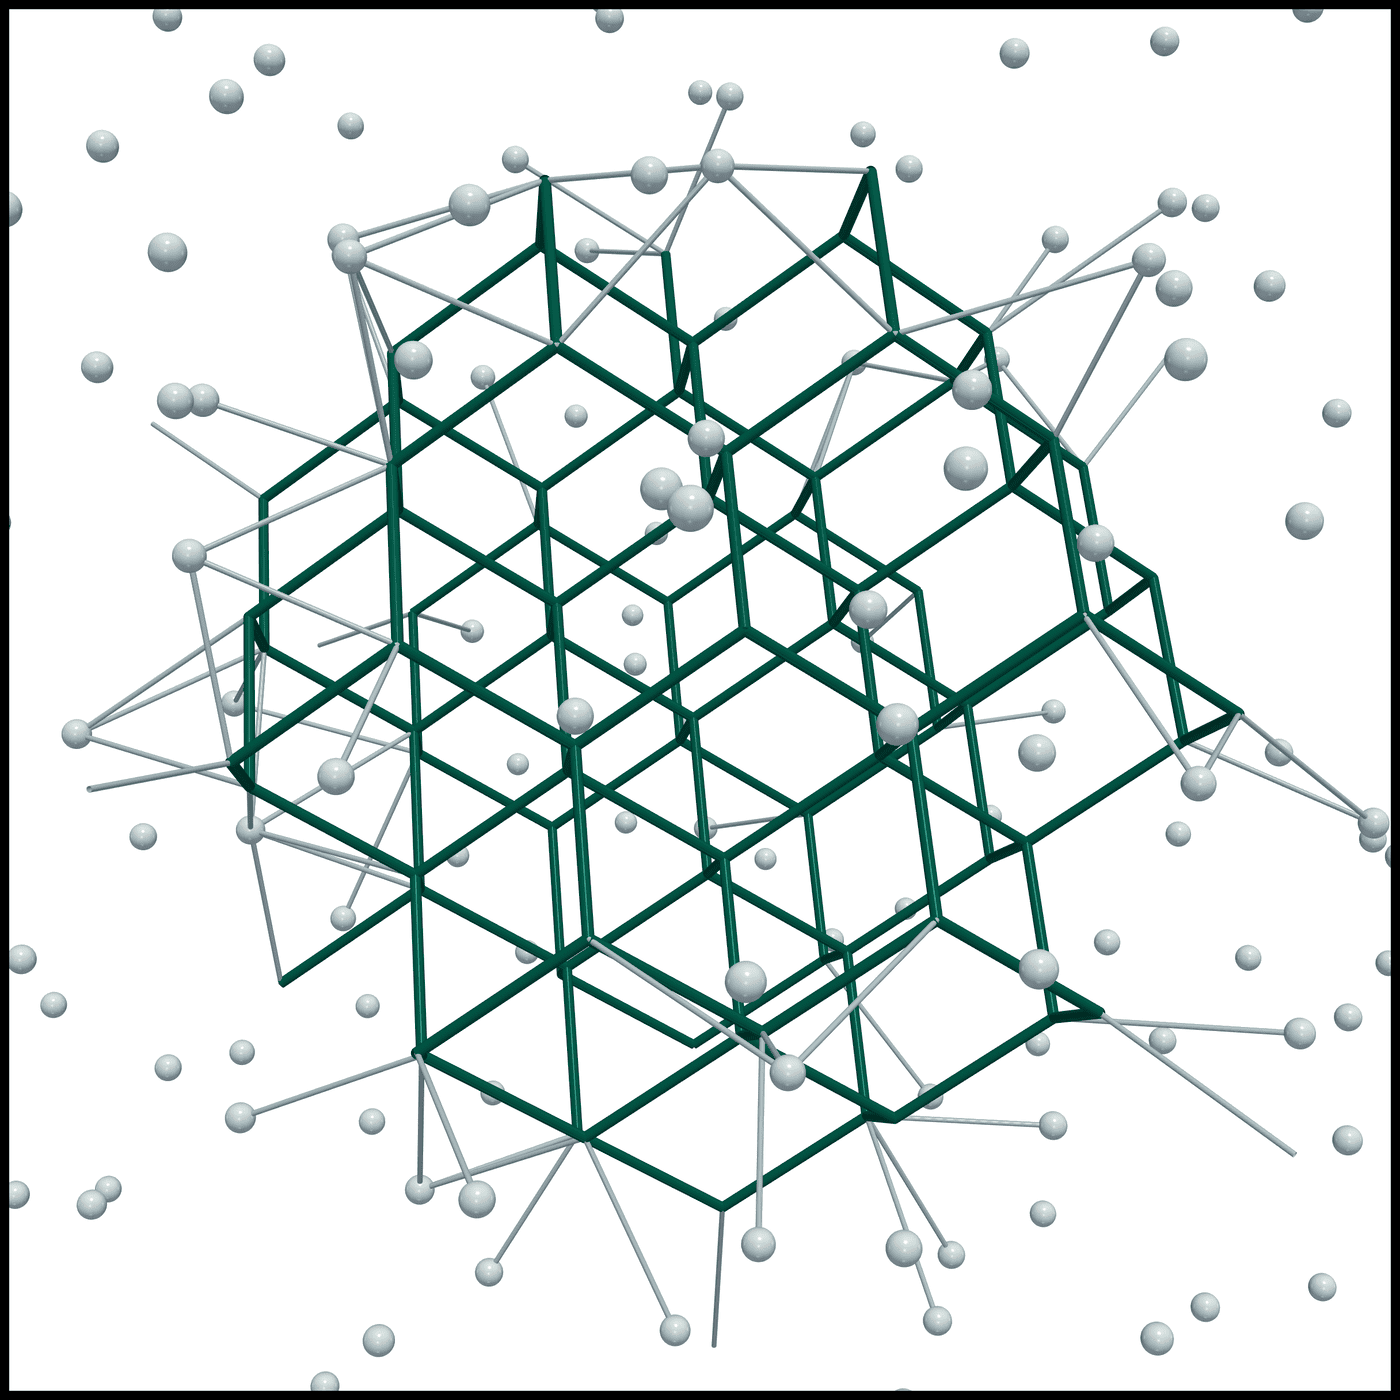
\includegraphics[height=5.2cm]{figures/seed_solvis_trim}
\caption{Spherical ice Ic seed in mW liquid, drawn with solvis.
Teal: $80$ seed oxygens and their first-shell edges.
Grey: liquid sites after the $2.6\,\mathring{\mathrm{A}}$ exclusion.
The production campaign uses the same cut at $4096$ liquid molecules.}
\label{fig:seed-xyz}
\end{figure}

A seeding run inserts an ice Ic sphere of \(N\) molecules into mW liquid (Figure~\ref{fig:seed-xyz}) and stops when the labelled cluster \(n_{\max}\) reaches \(2N\) or falls to \(20\).
The PLUMED action \texttt{DSEAMS\_CAGES} applies that rule inside LAMMPS every \(5\,\mathrm{ps}\).
Each seed size has twelve replicas in 4096 mW molecules.
The grown fraction rises above one half between 100 and 200 molecules at \(205\,\mathrm{K}\), between 200 and 300 at \(215\,\mathrm{K}\) and between 300 and 450 at \(225\,\mathrm{K}\) (record \texttt{elja-production}).
Twelve of twelve seeds of 700 molecules grow at every temperature.

On the last of the 148 stored frames of the 4096-molecule mW nucleation deposit \citep{goswami2020dseams}, the seeded cage assignment labels 995 molecules and places 905 in one cluster.
CHILL+ labels 497 molecules cubic or hexagonal and places 454 of them in one cluster (Figure~\ref{fig:app-nucleation}).
Across the deposit the largest CHILL+ cluster is \(0.24\) to \(0.50\) of the largest seeded cage cluster.

\begin{figure}[htbp]
\centering
\input{figures/app_nucleation}
\caption{Ice labels on the 148 stored frames of the 4096-molecule mW
nucleation deposit (figshare 11448702). Left: molecules labelled ice by
cage membership on the seeded four-nearest graph, by cage membership on
the $3.5\,\mathring{\mathrm{A}}$ cutoff graph, by CHILL+ (cubic plus
hexagonal) on the same cutoff graph, and by CHILL+ with the interfacial
label included. Right: the largest connected cluster $n_{\max}$ of each
ice label on its graph. Every point is one frame of the deposit; the
tables are \texttt{results/} of the reproducibility package
(\url{https://github.com/d-SEAMS/dseams2_repro}, \reproid).}
\label{fig:app-nucleation}
\end{figure}

On every public TIP4P/Ice nucleation dump of \citet{niu2019temperature} the cage assignment recovers the published fate of the nucleus (Figure~\ref{fig:app-public}).
The growing member of their critical-nucleus committor pair starts at \(n_{\max}=371\) and ends at 660, and the melting member starts at 384 and ends at 18.
CHILL+ places the two starting nuclei at 154 and 151 molecules.
A critical size stated in one coordinate therefore does not carry over to the other.

\begin{figure}[htbp]
\centering
\input{figures/app_public}
\caption{Largest ice cluster $n_{\max}$ by cage
membership on the seeded four-nearest graph, by cage membership on the
$3.5\,\mathring{\mathrm{A}}$ cutoff graph, and by CHILL+ (cubic plus
hexagonal). The plot covers every stored frame of the public TIP4P/Ice
nucleation dumps of Niu et al. The thin grey dashed line is $N_c=314$. The four-site dump is scored
on its oxygen sites.}
\label{fig:app-public}
\end{figure}

An ice/brine front with the Madrid-2019 ions \citep{zeron2019madrid} and TIP4P/2005 water starts from half a GenIce ice Ih block and a melted upper half (Figure~\ref{fig:app-brine-box}).
With no salt the labelled cluster grows over \(5\,\mathrm{ns}\) at \(230\), \(240\) and \(245\,\mathrm{K}\).
It starts at \(930\), \(939.5\) and \(927\) molecules and ends at \(1203.5\), \(1275\) and \(1319.5\) (means of two replicas).
With forty NaCl pairs it shrinks at all three temperatures, and no run ends with more than two ions in an all-ice shell.

\begin{figure}[htbp]
\centering
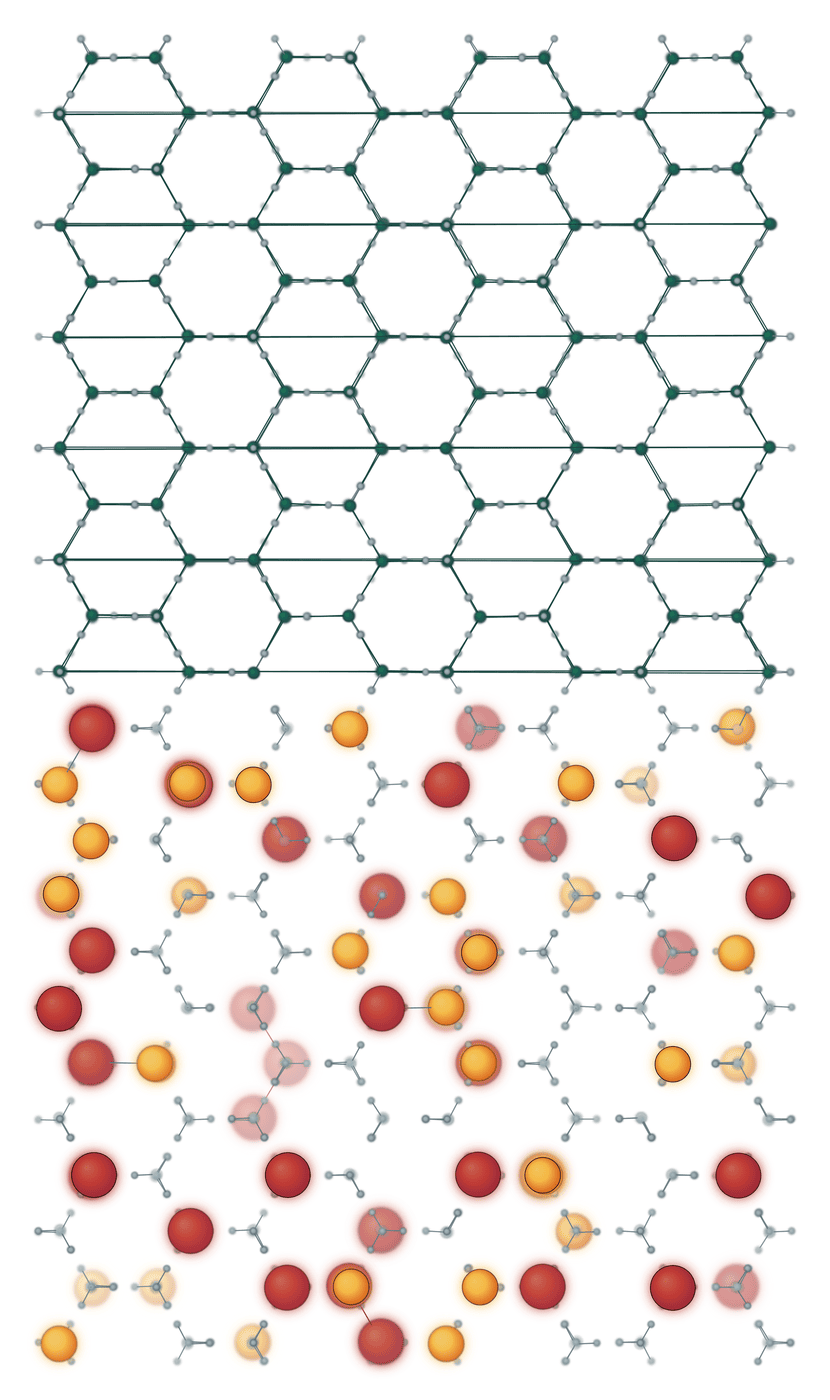
\includegraphics[height=6.4cm]{figures/brine_slab_xyzrender}
\caption{Ice/brine starting box of one $40$-pair replica,
$230\,\mathrm{K}$, $10\,\mathring{\mathrm{A}}$ slab, drawn with xyzrender \citep{xyzrender}.
Teal: ice oxygen network.
Grey: liquid water.
Coral: $\mathrm{Na}^{+}$.
Gold: $\mathrm{Cl}^{-}$.}
\label{fig:app-brine-box}
\end{figure}

On the ideal GenIce methane hydrates the ring-size signature search returns the \(16\) \(5^{12}\) and \(48\) \(5^{12}6^{2}\) cages of the \(2\times2\times2\) sI cell and the \(16\) \(5^{12}\) and \(8\) \(5^{12}6^{4}\) cages of the sII unit cell (Figure~\ref{fig:app-hydrate-box}).
Every cage holds one methane, no cage holds two and no methane is free.

\begin{figure}[htbp]
\centering
\begin{minipage}[b]{0.46\textwidth}
\centering
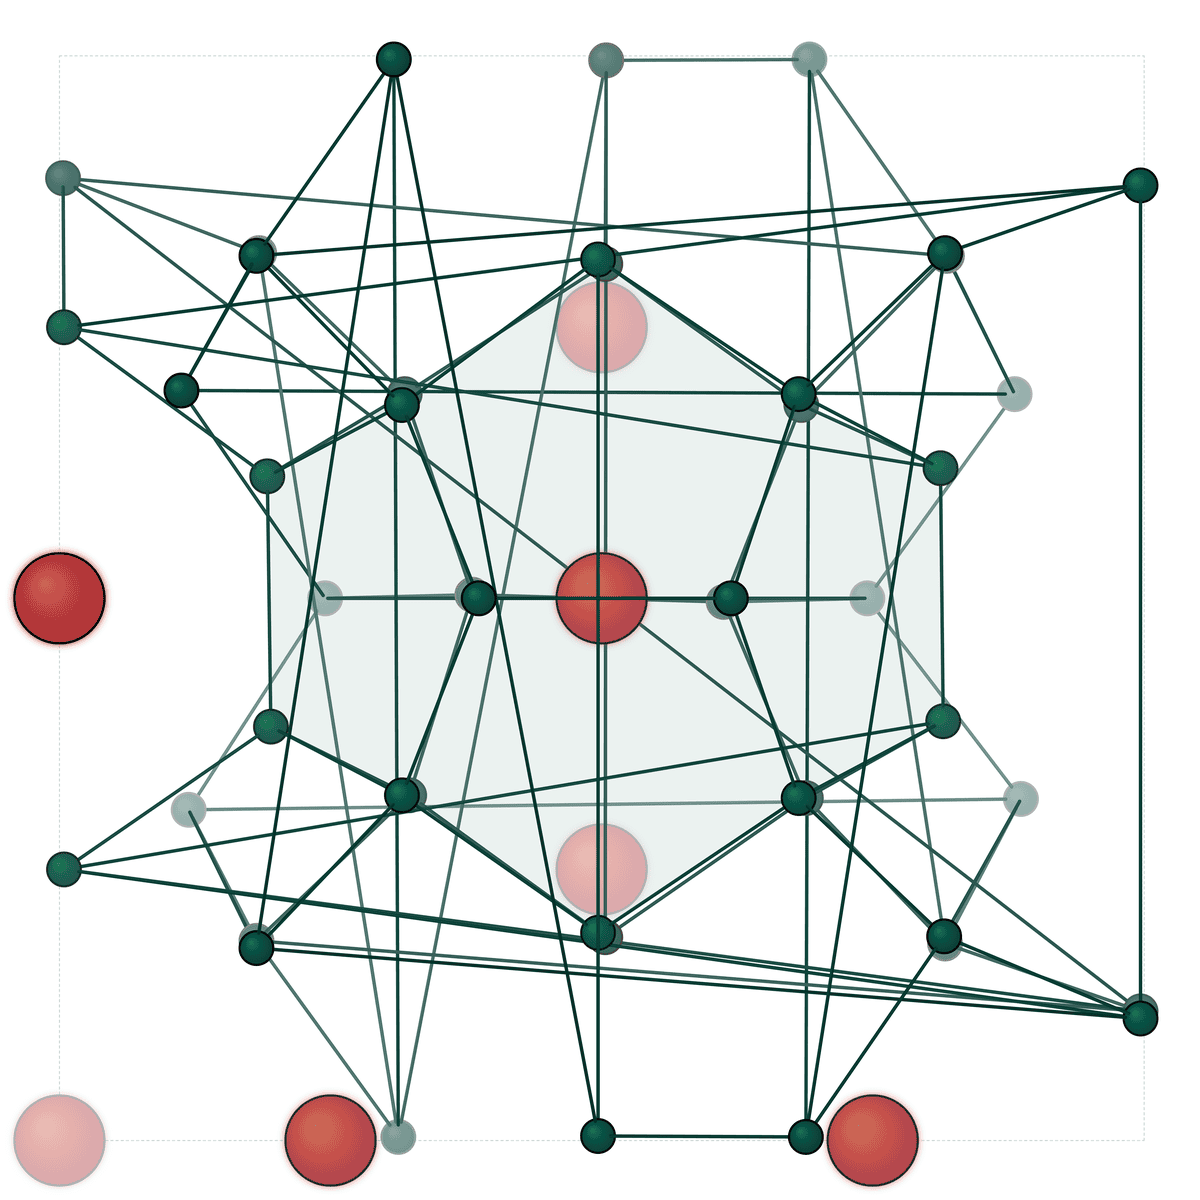
\includegraphics[height=5.0cm]{figures/si_hydrate_xyzrender}\\[0.3em]
{\small (a)}
\end{minipage}\hfill
\begin{minipage}[b]{0.46\textwidth}
\centering
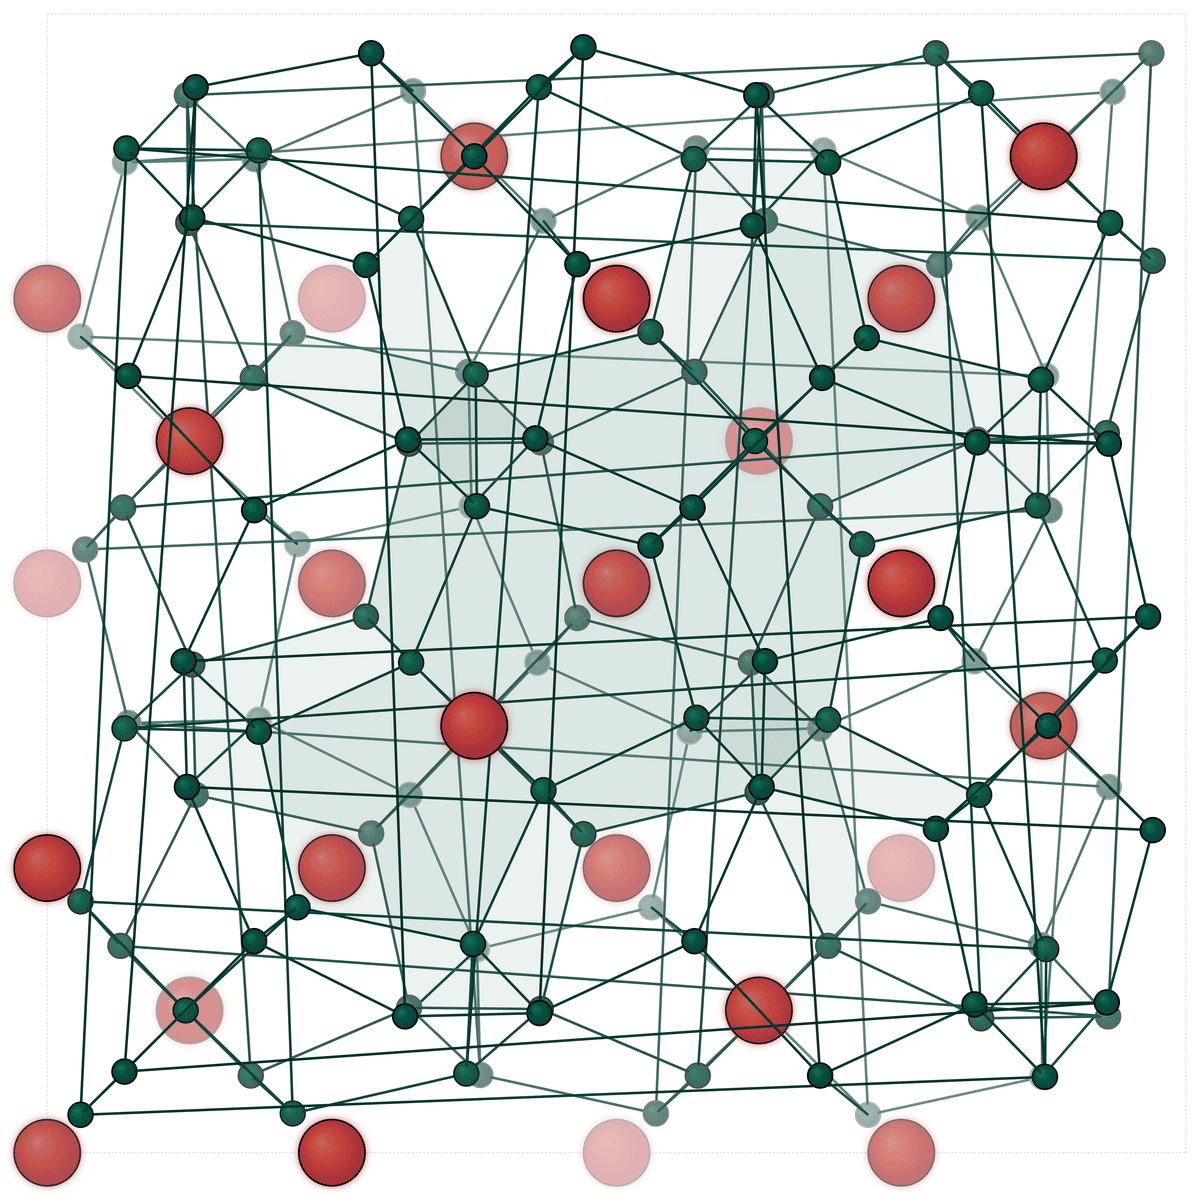
\includegraphics[height=5.0cm]{figures/sii_hydrate_xyzrender}\\[0.3em]
{\small (b)}
\end{minipage}
\caption{GenIce methane hydrates, unit cells drawn with xyzrender \citep{xyzrender}.
Teal: water oxygen network.
Pale hulls: five- and six-rings of the cages.
Coral: methane.
(a)~sI ($5^{12}$ and $5^{12}6^{2}$).
(b)~sII ($5^{12}$ and $5^{12}6^{4}$).}
\label{fig:app-hydrate-box}
\end{figure}

\section{Conclusions}
\label{sec:conclusions}
d-SEAMS 2.0 keeps the HC and DDC predicates of d-SEAMS 1 and evaluates them with shortest-path rings and an inverted atom-to-rings index.
Both the ring set and the cage flags update between frames, and each update returns the output of a rebuild.
A ring with no member within \(r\) hops of a changed bond keeps its status, with \(r=0\) up to seven members, and a cage flag outside two adjacency steps of a change keeps its value.
On one 4096-molecule crystal frame the ring and cage path takes \(46.8\,\mathrm{ms}\) against \(2.86\,\mathrm{s}\) for d-SEAMS 1.
With three changed bonds on a nucleation frame the ring update takes \(0.340\,\mathrm{ms}\) against \(12.878\,\mathrm{ms}\), and past a fixed fraction of changed atoms both updates switch to the batch pass.
Over a crystal trajectory the command line labels a frame 6.38 times faster than with a rebuild of every frame.
On deposited nucleation runs, where most bonds change between saved frames, it is at most 1.9\% slower than the rebuild.
On the same frames and core it returns the CHILL+ labels of OVITO, the \(q_6\) of freud, the rings and cages of GenIce2 and the ring census of RINGS.
We release d-SEAMS 2.0 as a C++20 library and command line under the MIT license as seams-core \coretag{} \citep{seamscore2026}, commit \texttt{305fb3c6} of \url{https://github.com/d-SEAMS/seams-core} with the ten patches of the program files.
The Python front end is PydSEAMSlib on PyPI \citep{pydseamslib2026}, and the Lua front end is yodaStruct \citep{yodastruct2026}.

\section*{CRediT authorship contribution statement}
Rohit Goswami: Conceptualization; Methodology; Software; Formal analysis; Writing -- original draft; Writing -- review \& editing.
Amrita Goswami: Conceptualization (original cage-membership assignment; confined topological criteria; seeding cluster and topological unit matching); Methodology; Software; Writing -- review \& editing.
Ruhila Goswami: Software (PydSEAMSlib, the Python bindings); Visualization (colour palette); Writing -- review \& editing.
Jayant K. Singh: Writing -- review \& editing.

\section*{Declaration of competing interest}
The authors declare no competing financial interests or personal relationships that influenced the work reported in this paper.

\section*{Funding}
This research did not receive any specific grant from funding agencies in the public, commercial, or not-for-profit sectors.

\section*{Code availability}
The engine is seams-core \coretag{} at \url{https://github.com/d-SEAMS/seams-core} \citep{seamscore2026}, source tree \coretree.
The Python interface is PydSEAMSlib \citep{pydseamslib2026}, at \url{https://github.com/d-SEAMS/PydSEAMSlib}.
It installs with \mbox{\texttt{pip install pydseamslib}} and loads with \mbox{\texttt{import pydseamslib}}.
This paper used PydSEAMSlib 2.11.1.
Its PyPI wheel wraps seams-core v2.11.0, and the records of Table~\ref{tab:compare} and of the label tests of Section~\ref{sec:accuracy} build its source distribution with seams-core \coretag{} as the engine.
The Lua front end is yodaStruct v2.10.0 \citep{yodastruct2026}.
The documentation is at \url{https://docs.dseams.info/}.

\section*{Data availability}
The reproducibility package \url{https://github.com/d-SEAMS/dseams2_repro} \citep{dseams2repro}, \reproid, fetches every public trajectory used here and checksums it.
These are the figshare deposits 11448702, 11448711, 11448720, 11448741 and 11448768 and Materials Cloud record 2020.0005/v1.
With the patch the package holds the workflow, the records of Tables~\sref{tab:records} and \sref{tab:records-full}, and the scripts that write the tables and figures from them.
The supplementary data hold the patch in \texttt{patches/} and the records dated 31 October 2026 in \texttt{repro-records/}.
The mW RINGS samples, their checksums and the commands that wrote them are the data deposit \texttt{10.5281/zenodo.TO-BE-MINTED} (placeholder DOI, TO-BE-MINTED, not published).
The rerun commands are in Section~\ref{sec:repro} and Section~\sref{sec:s-repro} of the supplement.

\section*{Declaration of generative AI and AI-assisted technologies in the manuscript preparation process}
Chatbots were used to refine certain turns of phrase and to speed through some implementation details; all the work is the authors' own.

\bibliographystyle{elsarticle-num-names}
\bibliography{dseams2}
\end{document}
